\artigotrue
\chapter{OPTIMIZATION OF SAMPLE CONFIGURATIONS FOR SPATIAL TREND ESTIMATION FOR SOIL MAPPING}
\chapternote{This chapter is based on the study \textit{spsann -- optimization of sample patterns using 
spatial simulated annealing}, presented at the EGU General Assembly 2015 \cite{Samuel-RosaEtAl2015a}, and 
\textit{Optimization of sample configurations for spatial trend estimation}, presented at Pedometrics 2015 
\cite{Samuel-RosaEtAl2015d}. Also collaborated in the preparation of this document: Dick J. Brus (Alterra, 
Wageningen University and Research Centre, the Netherlands), Gerard B. M. Heuvelink (ISRIC -- World Soil 
Information), Gustavo M. Vasques (Embrapa Soils, Brazil), and Lúcia Helena Cunha dos Anjos (Universidade 
Federal Rural do Rio de Janeiro, Brazil).}
\shorttitle{Sampling for the Spatial Trend}
\label{chap:chap08}

% \def\ptkeys{Recozimento simulado, Otimização multi-objetivo, Pareto, Amostragem por hipercubo latino 
% condicionado, Covariáveis}
% \begin{chapterabstract}{brazilian}{\ptkeys}
% Este é o resumo em português.
% \end{chapterabstract}

\def\enkeys{Simulated annealing. Multi-objective optimization. Pareto. Conditioned Latin hypercube sampling. 
Covariates}
  
\begin{chapterabstract}{english}{\enkeys}
The spatial trend is the part of a soil spatial model that deterministically explains the soil spatial 
variation using covariates. The sampling method most commonly used to identify and estimate the spatial trend 
is \emph{conditioned Latin hypercube sampling} (CLHS). In this study we propose conceptual and algorithmic 
improvements on CLHS, which are evaluated using synthetic data derived from a real-world  case study in Santa 
Maria, southern Brazil. The improvements include: 1) using the Pearson's $r$ only when all covariates are 
numeric, and the Cramér's $V$ when some or all covariates are factors, 2) defining marginal sampling 
strata using only the unique values of the sample quantiles estimated with a discontinuous function, and 3) 
scaling the objective functions to the same approximate range of values using the upper-lower bound approach 
with the Pareto maximum and minimum before aggregating them into a single utility function using a weighted 
sum. Compared to the original CLHS, our proposed modifications resulted in a sampling algorithm with an 
improved numerical behaviour, but this does not necessarily translates into improved prediction accuracy. 
Sample size has a larger influence on prediction accuracy than the sampling algorithm. However, 
optimizing sample configurations aiming at the association/correlation between covariates can degrade 
prediction accuracy.
\end{chapterabstract}

\formatchapter

\section{INTRODUCTION}
\label{sec:chap08-intro}

Modern soil mapping is based on using a model of spatial variation composed of two terms, 

\begin{equation}\label{eqn:chap08-lmm} % SEE IMAGE BELOW
 Y(\boldsymbol{s}) = m(\boldsymbol{s}) + e(\boldsymbol{s}).
\end{equation}

\def\footgerard{\footnote{Gerard Heuvelink shared the same opinion during his Richard Webster Medal speech at 
the conference of the Pedometrics Commission of the IUSS, which took place from 14--18 September 2015, in 
Córdoba, Spain.}}

\noindent The first term in the right-hand size in \autoref{eqn:chap08-lmm} is the spatial trend, 
which corresponds to the spatial variation of the soil property $Y(\boldsymbol{s})$ that is explained 
deterministically using spatially exhaustive covariates; the remaining spatial variation of 
$Y(\boldsymbol{s})$ is explained stochastically with the second term \cite{Cressie1993}. Soil scientists 
devoted all their attention to $m(\boldsymbol{s})$ for more than a century \cite{Jenny1961, Florinsky2012}. 
Post-war technological developments in the fields of mathematics, statistics, and informatics, made many soil 
scientists turn their focus to $e(\boldsymbol{s})$ \cite{WebsterEtAl1990}. Recent developments in remote 
sensing and machine-learning algorithms made those soil scientists shift their attention back to 
$m(\boldsymbol{s})$ \cite{MooreEtAl1993} -- but without forgetting $e(\boldsymbol{s})$ \cite{OdehEtAl1994} 
--, which now usually explains a considerably large proportion of the variation of $Y(\boldsymbol{s})$ 
compared to $e(\boldsymbol{s})$\footgerard. Besides, it is in $m(\boldsymbol{s})$ where we can incorporate 
most of our pedological knowledge \cite{Lark2012}.

Recent studies have shown that using more detailed covariates or more complex machine-learning algorithms can 
deliver more accurate soil maps, but the increase in prediction performance may be modest 
\cite{Samuel-RosaEtAl2015} and largely depends on the calibration data \cite{HeungEtAl2016}. Limited to the 
currently available covariates and machine-learning algorithms, and to the existing pedological knowledge, one 
of the major operational issues that needs to be solved in any soil mapping project is how to design an 
efficient spatial sample to estimate $m(\boldsymbol{s})$. The sampling method most commonly used to solve this 
problem is the \emph{conditioned Latin hypercube sampling} (CLHS). The CLHS was developed by Budiman Minasny 
and Alex McBratney at the University of Sydney in 2005, using an idea borrowed from the Latin hypercube 
sampling \cite{McKayEtAl1979, MinasnyEtAl2006b}. The popularity of the CLHS is due to its non-probabilistic 
nature, seen as a link with the sampling strategies used in \q{traditional soil survey}, easiness to 
implement, and the high flexibility which makes the addition of new features simple \cite{MinasnyEtAl2010a, 
RoudierEtAl2012, MulderEtAl2013, CarvalhoJuniorEtAl2014, CliffordEtAl2014}.

The CLHS is a heuristic strategy of creating spatial samples that aim at three objectives: ($\mathcal{O}_1$) 
uniform coverage of the marginal distribution of numeric covariates (continuous and discrete data, e.g. 
elevation, slope, etc.), ($\mathcal{O}_2$) proportional sample sizes for the classes of factor covariates 
(binary, categorical, and ordinal data, e.g. geology, land use, etc.), and ($\mathcal{O}_3$) reproduction of 
the linear correlation of numeric covariates. The main idea was that if a spatial sample reproduces the 
marginal distribution of the numeric and factor covariates, as well as the correlation matrix of the numeric 
covariates, it will approximately cover the multivariate distribution of the covariates -- this should put us 
closer to identifying the \q{true} spatial trend if we are (or assume to be) ignorant about its form.

Some critiques of the CLHS appeared in the literature since it was first published. Most of them focused on 
operational difficulties encountered in the field. For example, \citet{CambuleEtAl2013} argued that the 
CLHS is impractical in poorly-accessible areas, but \citet{RoudierEtAl2012} and \citet{MulderEtAl2013} showed 
that this is just a matter of how the algorithm is implemented. \citet{CliffordEtAl2014} presented an 
algorithm for selecting an alternative sampling point when a CLHS sample point is inaccessible. Only recently 
soil scientists started paying more attention to the theoretical and algorithmic aspects of the CLHS. 
\citet{MinasnyEtAl2010a} demonstrated that, given an assumed known linear spatial trend, the CLHS is 
suboptimal. \citet{CliffordEtAl2014} questioned the importance of meeting the third objective 
($\mathcal{O}_3$), as well as the mathematical approach used to find a solution for all three objectives 
jointly (see below). Finally, \citet{Brus2015} proposed an alternative method for selecting Latin hypercube 
samples with known inclusion probabilities so that these samples can also be used for design-based inference.

Our objective is to propose conceptual and algorithmic improvements on the CLHS, all of which we describe in 
the next section. We then evaluate if the proposed improvements result in a more accurate representation of 
the feature space and in more accurate spatial predictions.

\section{PROPOSED IMPROVEMENTS}

\subsection{Defining the Marginal Sampling Strata}

Given a \emph{numeric} covariate, CLHS uses the sample size $n$ to define the number of marginal 
sampling strata $c$, i.e. $c = n$, and the interpolated sample quantiles to define the breakpoints of the 
$c$ marginal sampling strata. The first objective of CLHS ($\mathcal{O}_1$) is to have exactly one 
sample point falling in each marginal sampling strata. However, depending on the level of discretization of 
the covariate values, CLHS may produce replicated breakpoints in the regions with a relatively high 
frequency of covariate values. For example, given a sample size of $n = 5$ and a covariate $\boldsymbol{a}$ 
with (ordered integer) values $\boldsymbol{a} = (1, 1, 1, 1, 2, 2, 3, 3, 4, 5, 8, 9, 9, 9, 9)$, the lower and 
upper boundaries of the $c = 5$ marginal sampling strata (mss) are $\boldsymbol{a}_{mss} = (1.0, 1.0, 2.6, 
4.4, 9.0, 
9.0)$. 
Because the marginal sampling strata in which a sample point $b_i$ falls is evaluated using the indicator 
function

\begin{equation*} % SEE IMAGE BELOW
 b_{sol_i} = 
 \begin{cases}
  1, & \text{if}\ a_{mss_j} \leq b_i \leq a_{mss_{j + 1}}\ \text{and}\ j = 1 \\ 
  1, & \text{if}\ a_{mss_j} < b_i \leq a_{mss_{j + 1}}\ \text{and}\ j > 1 \\ 
  0, & \text{otherwise}
 \end{cases}
\end{equation*}

\noindent where $i = 1, 2, \ldots, n$ refers to sample point candidates, and $j = 1, 2, \ldots, c$ to 
marginal sampling strata, the first and last marginal sampling strata (mms) of $\boldsymbol{a}$ will be empty, 
and the respective $n' = 2$ sample points will be allocated among the other three marginal sampling strata, 
with the set of allocation solutions $\boldsymbol{b}_{sol} = \{(0, 2, 1, 2, 0), (0, 1, 2, 2, 0), (0, 2, 2, 1, 
0)\}$. Ergo, CLHS will be unable to find the globally optimum allocation solution $\boldsymbol{b}_{sol} = (1, 
1, 1, 1, 1)$.

We propose defining the marginal sampling strata (mss) using only the unique values of the sample quantiles 
estimated with a discontinuous function \cite{HyndmanEtAl1996}. In our previous example, the strata boundaries 
would be $\boldsymbol{a}_{mss} = (1, 2, 4, 9)$. The number of sample points that should fall in each marginal 
sampling stratum is directly proportional to the number of sampling units (grids cells of a raster image) in 
that stratum of the covariate. For $\boldsymbol{a}$, this is $\boldsymbol{b}_{sol} = (2, 1, 2)$. The direct 
consequence of this modification is that, given a set of $p$ covariates, each of them will potentially have a 
different number of (quasi-equal-size) marginal sampling strata, i.e. $c_i \leq n$, where $i = 1, 2, \ldots, 
p$. This will ultimately depend on the shape of their empirical frequency distribution, on the level of 
discretization of the covariate values, and on the sample size $n$.

\subsection{Measuring the Association/Correlation Between Covariates}

Two of the objectives of CLHS ($\mathcal{O}_1$ and $\mathcal{O}_3$) are concerned with \emph{numeric} 
covariates, while only one ($\mathcal{O}_2$) focuses on \emph{factor} covariates. $\mathcal{O}_1$ and 
$\mathcal{O}_2$ are mathematically equivalent -- they aim at the coverage of the marginal distribution of the 
numeric and factor covariates, respectively --, and $\mathcal{O}_3$ measures the similarity between the 
population and sample correlation matrices of the numeric covariates as estimated with the Pearson's 
correlation coefficient $r$. The CLHS ignores the association among factor covariates, as well as among factor 
and numeric covariates. This means that CLHS gives more importance to numeric covariates. Such a bias cannot be 
corrected by simply attributing different \emph{weights} to each objective (see below).

To address the problem above we propose to replace Pearson's $r$ with Cramér's $V$

\begin{equation}\label{eqn:chap08-cramer} % SEE IMAGE BELOW
 V =  \sqrt{\frac{\chi^2 / n}{min(n_\text{col} - 1, n_\text{row} - 1)}},
\end{equation}

\noindent where $n_\text{row}$ and $n_\text{col}$ are the number of rows and columns of the bivariate 
contingency table, $n$ is the sample size, and $\chi^2$ is the chi-squared statistic

\begin{equation}\label{eqn:chap08-chi-squared} % SEE IMAGE BELOW
 \chi^2 = \sum_{i = 1}^{n_\text{row}}\sum_{j=1}^{n_\text{col}}\frac{(O_{ij} - E_{ij})^2}{E_{ij}},
\end{equation}

\noindent where $O_{ij}$ and $E_{ij}$ are the observed and expected frequencies, respectively, the marginal 
proportions of $O$ being the maximum likelihood estimates of the marginal proportions of $E$ 
\cite{Cramer1946, Agresti2002}. The Cramér's $V$ is a measure of association between factor covariates that 
ranges from $0$ to $+1$: the closer to $+1$, the larger the association between two factor covariates. 
Accordingly, the only requirement for using the Cramér's $V$ -- instead of the Pearson's $r$ -- is that any 
numeric covariate be transformed into a factor covariate, with the factor levels defined using the marginal 
sampling strata. One could still use the Pearson's $r$ when all covariates are numeric because computing the 
Cramér's $V$ is more computationally demanding.

\subsection{Aggregating the Objectives}

Sampling for spatial trend estimation is a \emph{multi-objective combinatorial optimization problem} (MOCOP): 
the spatial sample must meet a list of objectives among an almost infinite set of possible spatial samples. An 
important step for solving a MOCOP is to define each objective as a function, i.e. an \emph{objective function} 
$f_i$ \cite{Arora2011}. An $f_i$ associates a numerical value with each candidate spatial sample as a function 
only of the values of the $p$ covariates used to describe the spatial domain -- also known as \emph{design 
variables} \cite{Arora2011} -- at the $n$ sample points. The lower the objective function value, the closer the 
spatial sample is to meeting the respective objective. Thus, when solving a MOCOP, one aims at minimizing the 
vector of $k$ objective functions \cite{Arora2011}

\begin{equation}\label{eqn:chap08-mocop} % SEE IMAGE BELOW
 \boldsymbol{f}(\boldsymbol{X}) = (f_1(\boldsymbol{X}), f_2(\boldsymbol{X}), \ldots, f_k(\boldsymbol{X})),
\end{equation}\label{eqn:chap08-mocop}

\noindent where $\boldsymbol{X}$ is the design matrix, a $n \times p$ matrix subject to the implicit 
constraints imposed by the finiteness of the spatial domain and discreteness of the $p$ design variables. 
These implicit constraints define the set of values that can be assigned jointly to the design variables, i.e. 
the $p$-dimensional \emph{feasible design space} $\mathcal{S}$, which, in turn, defines the set of numerical 
values that can be returned by the objective functions, i.e. the $k$-dimensional \emph{feasible objective 
space} $\mathcal{Z}$ \cite{MarlerEtAl2004}.

Ideally, there is a traceable unique \emph{point cloud} $\boldsymbol{X}^*$ (i.e. a spatial sample with the 
values of the covariates at its sample points) that minimizes all objective functions simultaneously 
\cite{MarlerEtAl2009}. However, in practice such a unique point cloud seldom exists, and if it exists it is 
hard to find. In most cases there is a large set of optima point clouds that map onto a set of optima points 
on $\mathcal{Z}$ because, for example, multiple point clouds can return the very same objective function value 
\cite{Arora2011}. The set of optima point clouds is commonly defined using the concept of \emph{Pareto 
optimality} \cite{MarlerEtAl2004}: a point cloud $\boldsymbol{X}^*$ in $\mathcal{S}$ is Pareto optimum if and 
only if there is no other point cloud $\boldsymbol{X}$ in $\mathcal{S}$ that decreases the value of at least 
one objective function without increasing the value of another objective function.

A reasonable strategy to find a single optimum solution is to aggregate the objective functions into a single 
\emph{utility function} $U$ \cite{MarlerEtAl2005}. The most common aggregation method is the \emph{weighted 
sum} method, which is used in the CLHS. It employs weights to incorporate the \emph{a priori} preferences of 
the user, their relative values reflecting the importance of each objective function \cite{MarlerEtAl2009}. 
Thus, the MOCOP boils down to minimizing the \emph{convex} combination of objective functions

\begin{equation}\label{eqn:chap08-utility} % SEE IMAGE BELOW
 U = \sum_{i=1}^{k} w_i f_i(\boldsymbol{X}),
\end{equation}

\noindent where \emph{convex} means that the weights $w_i$ are constrained to $w_i > 0$ and $\sum_{i=1}^{k} w_i 
= 1$ \cite{MarlerEtAl2005, MarlerEtAl2009}. An important requirement of the weighted sum method is that the 
objective functions be scaled to the same approximate range of values so that any potential numerical dominance 
can be eliminated or minimized, and the weights can play the desired role \cite{MarlerEtAl2005, 
MarlerEtAl2009}. 

There are several methods to scale the objective functions \cite{MarlerEtAl2005}. The Fortran source code of 
CLHS shows that, although not mentioned in the original paper, CLHS scales $\mathcal{O}_1$ and $\mathcal{O}_3$ 
using the \emph{upper-bound approach}, $f_i'' =f_i(\boldsymbol{X}) / f_i^{max}$, where $f^{max}_{\mathcal{O}_1} 
= n \times p^{num}$ and $f^{max}_{\mathcal{O}_3} = 0.5p^{num^2} + p^{num}$, $p^{num}$ being the number of 
numerical covariates. $\boldsymbol{f}^{max}$ is a rough estimate of the single worst solution for 
$\mathcal{O}_1$ and $\mathcal{O}_3$, called the \emph{nadir point cloud} \cite{MarlerEtAl2004}. Thus, this 
transformation results in a non-dimensional objective function with an upper limit around 1, and its use is 
imposed due to the fact that, by definition, the three objective functions yield values of very different 
orders of magnitude: $\mathcal{O}_1$ > $\mathcal{O}_3$ > $\mathcal{O}_2$. This is because $\mathcal{O}_1$ uses 
the number of sample points per strata (0--$n$), while $\mathcal{O}_3$ uses the linear correlation coefficient 
(-1--1), and $\mathcal{O}_2$ uses the proportion of sample points per strata (0--1).

We believe that the \emph{upper-bound approach} is insufficient for a proper scaling of the objective functions 
because $\boldsymbol{f}^{max}$ usually is unattainable -- it does not correspond to any point cloud in 
$\mathcal{S}$ and/or is too far from the Pareto optimum set \cite{MarlerEtAl2004}. Defining 
$\boldsymbol{f}^{max}$ as the median of the objective functions over multiple spatial samples generated by 
simple random sampling \cite{CliffordEtAl2014} is a suboptimal strategy because it only ensures that the 
objective functions will have similar orders of magnitude at the beginning of the optimization, which might 
have a negligible influence in the definition of $\mathcal{Z}$ \cite{MarlerEtAl2005}. Besides, provided the 
optimization algorithm is well designed, the starting point should not influence the solution of the MOCOP (see 
below).

We propose using a more robust approach, i.e. the \emph{upper-lower bound approach},

\begin{equation}\label{eqn:chap08-pareto-min-max} % SEE IMAGE BELOW
 f_i'' = \frac{f_i(\boldsymbol{X}) - f_i^{\circ}}{f_i^{max} - f_i^{\circ}},
\end{equation}\label{eqn:chap08-pareto-min-max}

\noindent where $f_i^{\circ}$ is the \emph{utopia point}, the single best solution for the $i$th objective 
function, and $f_i''$ is the $i$th non-dimensional, scaled objective function constrained between zero and one 
\cite{MarlerEtAl2005}. Because of the above-mentioned problems regarding the definition of 
$\boldsymbol{f}^{max}$, it is more appropriate to use the \emph{Pareto maximum}, $f_i^{max} = max_{1 \leq j 
\leq k} f_ i(\boldsymbol{X}_j^*)$, where $\boldsymbol{X}_j^*$ is the point cloud that minimizes the $j$th 
objective function \cite{MarlerEtAl2005}. In practice, we optimize a sample configuration regarding each of the 
$k$ objective functions individually so that we end up with $k$ optimized sample configurations. The objective 
function value of each of the $k$ optimized sample configurations is recorded and set as the diagonal entries 
of the Pareto matrix $\varOmega$. Then, we take the $i$th optimized sample configuration and calculate the 
value of the $j$th objective functions, where $i \neq j$, and use the results as the off-diagonal entries of 
$\varOmega$. As such, $\varOmega$ is a $k \times k$ matrix with the objective function used to optimize the 
spatial sample in the columns, and the objective function used to calculate the objective function value in the 
rows. Finally, we lookup the columns of $\varOmega$ and record the largest absolute maximum observed in each of 
them, generally an off-diagonal entry. These are the Pareto maximum values of the $k$ objective functions. In 
turn, $f_i^{\circ}$ is replaced with the Pareto minimum, i.e. the smallest absolute minimum value observed in 
each column of $\varOmega$, generally the diagonal entry. This is because, like $\boldsymbol{f}^{max}$, 
$\boldsymbol{f}^{\circ}$ exists in the objective space $\mathcal{Z}$, but usually is unattainable, i.e. it does 
not correspond to any point cloud in $\mathcal{S}$ \cite{Arora2011}. The obvious drawback of this approach is 
the extra time needed to optimize each of the $k$ objective functions individually.

\subsection{Resulting Problem Definition}

Given the proposed modifications, the problem of sampling for spatial trend estimation for soil mapping is 
redefined using two objective functions,

\begin{equation}\label{eqn:chap08-corr} % SEE IMAGE BELOW
 \text{CORR} = \sum_{i=1}^{p}\sum_{j=1}^{p}|\varphi_{ij} - v_{ij}|,
\end{equation}

\noindent where $\varphi_{ij}$ and $v_{ij}$ are the population and sample associations (or correlations in case 
all covariates are numeric) at the $i$th row and $j$th column of the $p$-dimensional population and sample 
association (or correlation) matrices, and

\begin{equation}\label{eqn:chap08-dist} % SEE IMAGE BELOW
 \text{DIST} = \sum_{i=1}^{p}\sum_{j=1}^{c_i} |\pi_{ij} - \gamma_{ij}|,
\end{equation}

\noindent where $\pi_{ij}$ and $\gamma_{ij}$ are the proportion of sample and population points that fall in 
the $j$th class (or marginal sampling strata) of the $i$th covariate, $c_i$ being the number of classes of the 
$i$th covariate. With these two objective functions, we define a utility function $U$ as in 
\autoref{eqn:chap08-utility} aiming at a spatial sample that reproduces an 
\textbf{A}ssociation/\textbf{C}orrelation measure and the marginal \textbf{D}istribution of the 
\textbf{C}ovariates,

\begin{equation}\label{eqn:chap08-acdc} % SEE IMAGE BELOW
 \text{ACDC} = w_1\text{CORR} + w_2 \text{DIST},
\end{equation}

\noindent with $w_1 = w_2 = 0.5$ when we do not have \emph{a priori} preferences towards the objective 
functions.

\section{CASE STUDY}

We developed a  case study to evaluate the proposed improvements and compare them with the original CLHS. It 
was based on using synthetic data derived from a real-world  case study \cite{Samuel-RosaEtAl2015}. The study 
site is a small catchment of about \SI{2000}{\hectare} located on the southern edge of the Plateau of the 
Paraná Geologic Province, Rio Grande do Sul, Brazil. The real-world dataset contains $n = 350$ point soil 
observations of the topsoil, and includes several soil properties, but only bulk density data 
(BUDE,~$\si{\mega\gram\per\metre\cubic} \times 100$) was used ($n = 282$). The dataset also includes several 
covariates derived from area-class soil maps, digital elevation models, geological maps, land use maps, and 
satellite images. All processing steps used to derive the covariates were described by 
\citet{Samuel-RosaEtAl2015}.

\subsection{Soil Data Generating Process}
\label{sec:chap08-simulation}

In an ideal world, we would create $\mathcal{R} \geq 100$ spatial samples of $\mathcal{N} \geq 2$ sizes with 
each of the $\mathcal{A} \geq 2$ algorithms that we want to compare. Then we would go to the field, sample the 
soil, and measure a property to construct $\mathcal{D} = \mathcal{R} \times \mathcal{N} \times \mathcal{A}$ 
calibration datasets. The same property would be measured at a fixed set of probabilistically selected 
validation sites. Each calibration dataset would be used to calibrate a model, with which we would predict at 
the validation sites. The $\mathcal{A}$ sampling algorithms would then be compared on how well 
they performed, for each of the $\mathcal{N}$ sizes, using the confidence interval of a prediction error 
statistic over all $\mathcal{R}$ spatial samples. In such an experiment, the random selection of spatial 
samples would be the \emph{source of variation} \cite{deGruijterEtAl1990}.

In the real world\dots Due to limited resources, we created only $\mathcal{R} = 1$ spatial sample with 
$\mathcal{N} = 3$ sizes with each of the $\mathcal{A} = 4$ sampling algorithms to be compared (CORR, DIST, 
ACDC, and CLHS). The variation in the experiment had to come from another source: we chose it to be the soil 
property data. We did so using unconditional sequential Gaussian simulation \cite{Goovaerts2001, Pebesma2004}. 
To start, we defined a theoretical (or super-population) model, our \emph{soil data generating process}, which 
should be as close to reality as possible. Thus, the soil data generating process was defined empirically by 
calibrating a (non)linear mixed model to the observed (real) BUDE data. The main calibration steps were as 
follows \cite{Breiman2001, LiawEtAl2002, DiggleEtAl2007, Lark2012}:

\begin{enumerate}[label = (\Roman*)]
\item Random forest regression: grow $n_{\text{trees}} = 500$ regression trees with a maximum terminal node 
size of $n_{\text{node size}} = 5$ points, each tree grown using $n = 282$ calibration points randomly selected 
with replacement (bootstrap sample) from the set of $n = 282$ point soil observations (about $n_{\text{in-bag}} 
= n \times \left(1 - \left(\frac{n - 1}{n}\right)^{n}\right) = 178$ unique point soil observations), and 
$p_{\text{in-bag}} = 4$ covariates randomly selected at each split out of a set of $p = 12$ covariates 
(\texttt{SOIL\_25c}, \texttt{SOIL\_25h}, \texttt{SOIL\_25j}, \texttt{LU2009a}, \texttt{LU2009b}, 
\texttt{LU2009d}, \texttt{GEO\_50c}, \texttt{RED\_30}, \texttt{ELEV\_90}, \texttt{SLP\_90\_15}, 
\texttt{NOR\_90\_127}, \texttt{NOR\_90\_255}) selected and described as in \citet{Samuel-RosaEtAl2015}.

\item Out-of-bag predictions: use each of the $n_{\text{trees}} = 500$ regression trees from step (1) to 
predict BUDE at the point soil observations not included (out-of-bag) in the respective calibration dataset 
(about $n_{\text{out-of-bag}} = n - n_{\text{in-bag}} = 104$ point soil observations), and compute the average 
of the predicted BUDE at each point soil observation (about $n_{\widehat{BUDE}} = n_{\text{trees}} \times 
\left(\frac{n - 1}{n}\right)^{n} = 184$ predicted values for each out-of-bag point).

\item Linear mixed model: assume that the average of the out-of-bag predictions from step (2) are linearly 
related to BUDE and present insignificant conditional bias, and use them as a covariate in the fixed effects of 
a linear mixed model (LMM), the random effects modelled using the Whittle-Matérn model, all parameters being 
estimated by Gaussian restricted maximum likelihood (REML).
\end{enumerate}

The parameters of the LMM are the coefficients $\beta_0$ and $\beta_1$ of the linear trend, which correct any 
linear bias in the random forest regression out-of-bag predictions \cite{LiawEtAl2002}, and the nugget 
($\tau^2$), sill ($\sigma^2$), and range ($\alpha$) of the Whittle-Matérn model. The shape parameter ($\nu$) of 
the Whittle-Matérn model was defined separately, by choosing from a set of discrete values $\nu = (0.5, 1.0, 
2.0, 4.0, 8.0)$ based on the resulting profile likelihood for $\nu$ and maximized restricted log-likelihood, 
and on the computing time \cite{Stein1999, DiggleEtAl2007}. The fitted LMM ($\beta_0 = 
\SI{13.35}{\mega\gram\per\cubic\metre}$, $\beta_1 = 0.91$, $\tau^2 = 
\SI{349.51}{\mega\gram\per\metre\tothe{6}}$, $\sigma^2 = \SI{97.24}{\mega\gram\per\metre\tothe{6}}$, $\alpha = 
\SI{210.99}{\metre}$, $\nu = 2.0$) explained \num{38} and \SI{18}{\percent} of the sample variance of BUDE with 
$m(\boldsymbol{s})$ and $e(\boldsymbol{s})$, respectively (\autoref{fig:chap08-bude-vario}).

\begin{figure}[!ht]
 \centering
 \begin{minipage}{0.60\textwidth}
  \subcaption{}
  \centering
  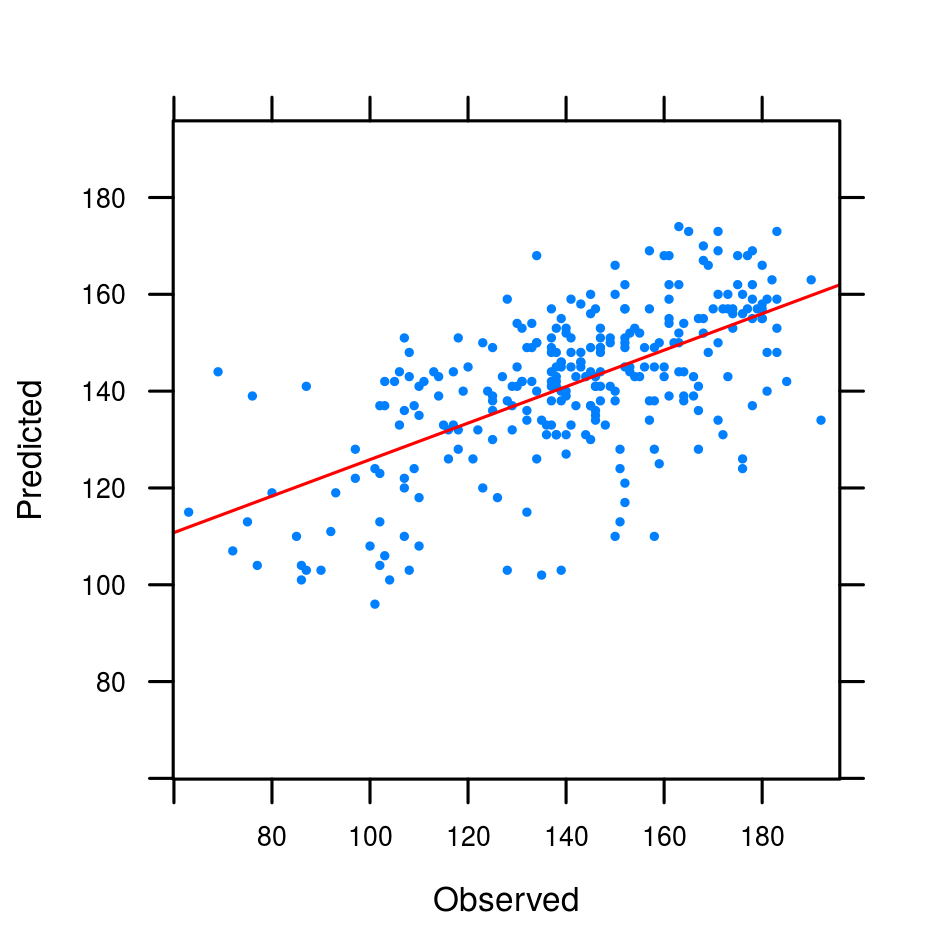
\includegraphics[width = \textwidth]{fig/chap08-random-forest-fit}
 \end{minipage}
 \begin{minipage}{0.60\textwidth}
  \centering
  \subcaption{}
  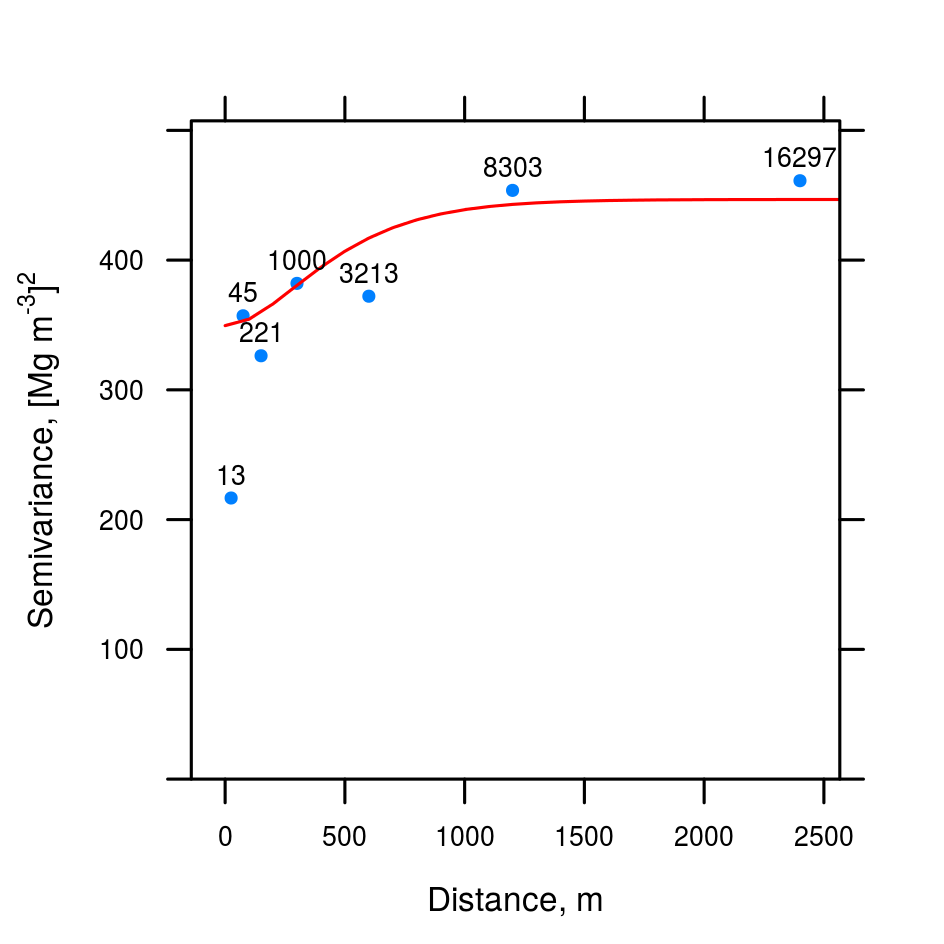
\includegraphics[width = \textwidth]{fig/chap08-bude-vario}
 \end{minipage}
 \caption[(Non)Linear mixed model fitted to the soil bulk density data.]{(Non)Linear mixed model fitted to the 
 soil bulk density data (BUDE, $\si{\mega\gram\per\cubic\metre} \times 100$) measured at $n = 282$ 
calibration locations. The top panel shows the relation between out-of-bag random regression forest 
predictions and BUDE, here representing the deterministic component $m(\boldsymbol{s})$. The bottom panel shows 
the restricted maximum likelihood fit of the variogram model (red line) to BUDE, i.e. the stochastic component 
$e(\boldsymbol{s})$. Exponentially spaced lag-distance classes are used to depict the sample variogram (blue 
dots) along with the number of point-pairs in each variogram lag-distance class.}
 \label{fig:chap08-bude-vario}
\end{figure}

With the random forest regression and the LMM at hand, we produced $\mathcal{R} = 1000$ equiprobable 
realizations of an isotropic Gaussian random field of BUDE. Each realization is constituted of a collection of 
BUDE values at a fine grid of \num{\sim800000} regularly spaced (\SI{5}{\metre}) points covering the entire 
study area. Because we used \emph{unconditional} Gaussian simulation -- a simulation that is only 
\emph{globally} conditioned to the histogram (and variogram) of the data observed at the calibration locations 
\cite{Goovaerts1997} -- and a large number of realizations, we expected to find the whole set of possible BUDE 
values (i.e. the global histogram) at any point of the simulation grid, over the $\mathcal{R} = 1000$ 
realizations. Thus, the variance -- our uncertainty -- is the same everywhere. This is in contrast with 
\emph{conditional} Gaussian simulation -- a simulation that is \emph{locally} conditioned to the data observed 
at the calibration locations --, which serves the purposes of honouring the data at the calibration locations, 
thus reducing the variance of the output realizations \cite{Goovaerts1997}. In our study, \emph{conditional} 
Gaussian simulation is inappropriate as a model of uncertainty because the sampling algorithms that we evaluate 
are designed to situations where we know very little, everywhere, about the spatial structure of the soil data 
generating process.

Unconditional simulation algorithms approximate the globally conditioned distribution of a soil variable at a 
given point using neighbouring simulated values as local conditioning information \cite{Goovaerts1997}: the 
larger the neighbourhood, the better the approximation. A sensible criterion to select the nearest simulated 
values is the practical range of the variogram model. However, as the simulation proceeds, the number of 
simulated values within this neighbourhood becomes computationally prohibitive \cite{Goovaerts1997, 
WebsterEtAl2007, Pebesma2013}. Thus, we used a fixed maximum number of simulated values $n_{max} = 100$ within 
the practical range of the variogram model (\SI{1132.657}{\m}) that are closest to the point being simulated. 
Last, but not least, sequential simulation algorithms speed up computations by using the same random path in 
all simulations, allowing it to reuse the \q{expensive results}: neighbourhood selection and solution to the 
kriging equations \cite{Goovaerts1997, WebsterEtAl2007, Pebesma2013}. We believe that following the same random 
path to generate each of the $\mathcal{R} = 1000$ realizations can introduce a structural component in the 
approximation errors. To avoid that, simulations were carried out in five batches of $\mathcal{R} = 250$ 
realizations using a different seed for the pseudo-random number generators each time.

\subsection{Spatial Sampling}

We compared $\mathcal{A} = 4$ criteria (CORR, DIST, ACDC, and CLHS) for optimizing sample configurations for 
spatial trend estimation for soil mapping using $\mathcal{N} = 3$ sample sizes $n = (100, 200, 400)$. These 
sample sizes correspond to the moderately high inspection density (1 sample point per 20, 10, and 
\SI{5}{\hectare}, respectively) recommended for the production of soil maps published at a \scale{25000} 
\cite{Rossiter2000}. Spatial sample configurations were optimized regarding each of the four criteria using 
\textbf{sp}atial \textbf{s}imulated \textbf{ann}ealing as implemented in the \texttt{spsann} package for 
\texttt{R}, designed specifically for the purpose of this study and made available in The Comprehensive R 
Archive Network (\cran).

\subsubsection{Spatial simulated annealing}
\label{sec:chap08-spsann}

Simulated annealing is a popular method with widespread use to solve combinatorial optimization problems in the 
soil and geosciences such as stochastic simulation \cite{Deutsch1992, Goovaerts2000}, estimation of model 
parameters \cite{LarkEtAl2003}, resource allocation and land use planning \cite{MuttiahEtAl1996, AertsEtAl2002, 
DuhEtAl2007}, and spatial sampling and monitoring \cite{vanGroenigenEtAl1997, SimbahanEtAl2006, BrusEtAl2007a, 
MarchantEtAl2006, MinasnyEtAl2006b, MellesEtAl2011}. This is mainly due to its robustness against local optima 
and easiness of implementation \cite{MetropolisEtAl1953, KirkpatrickEtAl1983, Cerny1985, AartsEtAl1989, 
Groenigen1999a}.

Simulated annealing is a heuristic algorithm that sequentially searches for the optimum solution for the 
problem at hand using the information \q{learned} from randomly trying solutions out of a large set of possible 
solutions, i.e. by trial and error. In spatial sampling, this means sequentially trying out randomly selected 
sample configurations $\boldsymbol{X}$ and checking how well they conform to the chosen criterion. Every time 
the newly selected sample configuration $\boldsymbol{X}_{i + 1}$ returns an improved (lower) objective function 
value $\boldsymbol{f}(\boldsymbol{X}_{i + 1})$ than the previously selected sample configuration 
$\boldsymbol{X}_i$, the latter is immediately discarded in favour of the former. The set of formal rules used 
to generate a new sample configuration $\boldsymbol{X}_{i + 1}$ to be compared with $\boldsymbol{X}_i$ with 
respect to the chosen criterion is called the \emph{generation mechanism} \cite{Groenigen1999a, BrusEtAl2007a, 
WebsterEtAl2013}.

The generation mechanism fundamentally works by means of randomly perturbing $\boldsymbol{X}_i$, specifically 
by adding random noise to the x- and y-coordinates of one of the sample points of $\boldsymbol{X}_i$. We call 
this process \emph{jittering}. The main requirement is that the minimum ($x_\text{min}$ and $y_\text{min}$) and 
maximum ($x_\text{max}$ and $y_\text{max}$) quantity of random noise that can be added to the x- and 
y-coordinates of a sample point be specified. These will define the \emph{neighbourhood} within which a sample 
point can be moved around. This neighbourhood corresponds to a rectangle centred at the sample point, with 
sides proportional to the sides of the rectangle that spans the sampling region. $x_\text{max}$ and 
$y_\text{max}$ should be large enough to enable all sample points visiting (almost) any place in the sampling 
region during the optimization such that the starting sample configuration -- generally obtained by simple 
random sampling -- has no direct influence on the final sample configuration.

Adding random noise to the x- and y-coordinates of a sample point corresponds to selecting a candidate location 
in the neighbourhood. This can only be done after the set of \emph{effective} candidate locations has been 
identified, i.e. after the presence of non-sampling areas (e.g. buildings and water bodies), as well as the 
shape and finiteness of the sampling region have been taken into account. Using a \emph{finite} set of 
candidate locations is an efficient way of achieving this because, by definition, the candidate location will 
always fall within the sampling region and out of non-sampling areas. A finite set of candidate locations is 
created by discretizing the sampling region beforehand, that is, by creating a fine grid of points that serve 
as candidate locations during the entire search for the optimum sample configuration. To minimize its 
disadvantages -- such as the fact that not all locations in the sampling region can enter the sample -- one can 
see the fine grid of points as the centre nodes of a finite set of grid cells and use a form of \emph{two-stage 
random sampling} \cite{WalvoortEtAl2010}: first, one of the candidate \q{grid cells} is selected with 
replacement in the neighbourhood, i.e. independently of already being occupied by another sample point; then, 
the candidate location for the sample point is selected within that \q{grid cell} by simple random sampling.

However, to be able to escape from apparently optima solutions that appear too early during the search to be 
true -- local optima solutions --, the newly selected sample configuration $\boldsymbol{X}_{i + 1}$ can be 
accepted even if it returns an inferior objective function value, i.e. $\boldsymbol{f}(\boldsymbol{X}_{i + 1}) 
>  \boldsymbol{f}(\boldsymbol{X}_i)$. This means that the algorithm \q{understands} that taking a step back 
sometimes during the search can lead to better results. The decision whether to accept or not a sample 
configuration is described by the Metropolis criterion \cite{MetropolisEtAl1953}, used to compute the 
\emph{acceptance probability} $P(\boldsymbol{X}_i \rightarrow \boldsymbol{X}_{i + 1})$ as

\begin{equation}\label{eqn:chap08-metropolis} % SEE IMAGE BELOW.
 P(\boldsymbol{X}_i \rightarrow \boldsymbol{X}_{i + 1}) = 
 \begin{cases}
  1, & \text{if}\  \boldsymbol{f}(\boldsymbol{X}_{i + 1}) \leq  \boldsymbol{f}(\boldsymbol{X}_i), \\ 
  exp\left(\frac{\boldsymbol{f}(\boldsymbol{X}_i) -  \boldsymbol{f}(\boldsymbol{X}_{i + 1})}{T}\right),  
      & \text{if}\  \boldsymbol{f}(\boldsymbol{X}_{i + 1}) >  \boldsymbol{f}(\boldsymbol{X}_i ),
 \end{cases}
\end{equation}

\noindent where $T$ is a positive control parameter that dictates how likely it is that an inferior sample 
configuration will be accepted.

Parameter $T$, traditionally called the \emph{temperature} parameter, is at the core of simulated annealing. 
This is because simulated annealing tries to mimic the process used in metallurgy and materials science known 
as \emph{annealing}, by which a molten metal is scheduled to gradually cool so that its solidifications results 
in such an arrangement of the atoms that form a perfect, minimum energy, mechanically resistant, crystalline 
structure \cite{MetropolisEtAl1953, KirkpatrickEtAl1983, Cerny1985}. A closer example is the formation of 
extrusive (volcanic) igneous rocks by the cooling of effusive lava, where the cooling rate strongly determines 
the size of crystals in the resulting rock \cite{HaldarEtAl2014}: sudden cooling (seconds, minutes) of lava 
creates amorphous volcanic glass with vitreous texture such as pumice; slower cooling (hours, weeks) enables 
the growth of crystals, which can sometimes be visible to the naked eye, resulting in more mechanically 
resistant rocks such as basalt. Much larger crystals will be observed in intrusive (plutonic) igneous rocks 
such as granite, but their growth is due to a very slow cooling of magma, sometimes thousands or millions of 
years \cite{HaldarEtAl2014}.

As the concept of temperature says, what happens at the atomic level during the cooling process of a molten 
metal (or lava and magma) is the reduction of the average kinetic energy -- the energy of motion -- of the 
particles. When optimizing spatial samples using simulated annealing, high \q{kinetic energy} means that 1) 
considerably different sample configurations might be tried out every time, and 2) it is very likely that 
inferior sample configuration will be accepted. As the \q{kinetic energy} decreases, the difference between 
$\boldsymbol{f}(\boldsymbol{X}_{i + 1})$ and $\boldsymbol{f}(\boldsymbol{X}_i)$ will be smaller, as well as 
the probability of accepting $\boldsymbol{f}(\boldsymbol{X}_{i + 1})$ if it is inferior to 
$\boldsymbol{f}(\boldsymbol{X}_i)$. To control this in practice, one needs to set up an annealing schedule.

The \emph{annealing schedule} corresponds to the set of formal rules that determine how the probability of 
accepting inferior sample configurations is decreased as the search for the globally optimum sample 
configuration evolves \cite{AartsEtAl1989, Groenigen1999a, WebsterEtAl2013}. When optimizing the configuration 
of a spatial sample, we have to decide upon a feasible annealing schedule, i.e. a schedule that enables finding 
the globally optimum sample configuration (or a sample configuration very close to it) in a reasonable amount 
of time. For that end, a large initial value of $T$ is chosen by trial and error so that almost all sample 
configurations tried out during the first temperature step are accepted. A temperature step, more precisely a 
\emph{Markov chain}, corresponds to the series of tryouts made with a constant value of $T$. The number of 
tryouts made with a constant value of $T$ corresponds to the length of a Markov chain $chain_\text{length}$, 
which should be long enough so that the \q{system} will tend to a \q{kinetic equilibrium}.

In practice, the length of a Markov chain has to be limited, and the equilibrium can only be approximated 
\cite{WebsterEtAl2013}. The only requirement is that every point be jittered at least once as it would happen 
with the atoms in a physical system \cite{MetropolisEtAl1953}. To initiate a new Markov chain $j + 1$, one 
reduces $T$ linearly by a control parameter $\delta_{T}$, with $0 < \delta_{T} < 1$, so that $T_{j + 1} = 
\delta_{T}T_j$ \cite{AartsEtAl1989}. The same applies to the generation mechanism by using a decrement function 
to reduce the size of the neighbourhood as the search for the optimum sample configuration evolves. The reason 
for this is that, as the search evolves and approaches its end, it is likely that moving a sample point over a 
short distance contributes more to finding the global optimum than moving it over larger distances 
\cite{GroenigenEtAl1998}. The decrement function determines that the size of the neighbourhood is reduced 
linearly at the end of the $j$th chain. For the x-axis of the neighbourhood,

\begin{equation} % SEE IMAGE BELOW
x_{\text{max}_{j + 1}} = x_{\text{max}_{j = 0}} - \frac{j}{n_\text{chains}} \times x_{\text{max}_{j = 0}} - 
                                           x_\text{min} + x_\text{dim},
\end{equation}

\noindent where $x_{\text{max}_{j + 1}}$ is the dimension of the x-axis of the neighbourhood in the next chain,
i.e. the maximum allowed shift in the x-coordinate, $x_{\text{max}_{j = 0}}$ is the dimensions of the x-axis
of the neighbourhood in the first chain, $x_\text{min}$ is the minimum required shift in the x-coordinate, 
$x_\text{dim}$ is the grid spacing in the x-coordinates, and $n_\text{chains}$ is the maximum affordable total 
number of Markov chains (the very same applies to the y-axis of the neighbourhood). The maximum affordable 
total number of Markov chains $n_\text{chains}$ has to be large enough such that the globally optimum sample 
configuration can be found. Finally, one or more criteria for stopping the search can be defined, such as the 
maximum affordable number of Markov chains completed without returning an improved sample configuration 
$n_\text{chain stop}$ \cite{Groenigen1999a}.

% \noindent and 

% \begin{equation} % SEE IMAGE BELOW
% y_{\text{max}_{j + 1}} = y_{\text{max}_{j = 0}} - \frac{j}{n_\text{chains}} \times y_{\text{max}_{j = 0}} - 
%                                            y_\text{min} + y_\text{dim},
% \end{equation}

% \noindent where $x_{\text{max}_{j + 1}}$ and $y_{\text{max}_{j + 1}}$ are the dimensions of the neighbourhood 
% in the next chain, i.e. the maximum allowed shifts in the x- and y-coordinates, $x_{\text{max}_{j = 0}}$ and 
% $y_{\text{max}_{j = 0}}$ are the dimensions of the neighbourhood in the first chain, $x_\text{min}$ and 
% $y_\text{min}$ are the minimum required shifts in the x- and y-coordinates, $x_\text{dim}$ and $y_\text{dim}$ 
% are the grid spacings in the x- and y-coordinates, i.e. the grid cell size, and $n_\text{chains}$ is the 
% maximum affordable total number of Markov chains. The maximum affordable total number of Markov chains 
% $n_\text{chains}$ has to be large enough such that the globally optimum sample configuration can be found. 
% Finally, one or more criteria for stopping the search can be defined, such as the maximum affordable number of 
% Markov chains completed without returning an improved sample configuration $n_\text{chain stop}$ 
% \cite{Groenigen1999a}.

All parameters of the generation mechanism ($x_\text{min}$, $y_\text{min}$, $x_\text{max}$ and $y_\text{max}$) 
and annealing schedule ($chain_\text{length}$, $n_\text{chains}$, and $n_\text{chain stop}$) have to be defined 
by trial and error, and based on the current knowledge and available resources \cite{WebsterEtAl2013}. A useful 
tool is a plot with the evolution of the objective function values as measured at the end of each Markov chain 
\cite{LarkEtAl2003}: objective function values should present large fluctuation during the first Markov chains, 
then gradually stabilize and decrease till a minimum is reached at which they remain for $n_\text{chain stop}$ 
Markov chains.

\subsubsection{Experimental design}

In this study, we used an annealing schedule with a maximum affordable total number of Markov chains 
$n_\text{chains} = 500$ without imposing any stopping criterion. The initial temperature $T$ was set such that 
more than \SI{95}{\percent} of the tryouts during the first Markov chain would be accepted. To initiate a new 
Markov chain $j + 1$, $T$ was linearly decreased by a factor of $\delta_{T} = 0.95$. The length of each Markov 
chain was set to $chain_\text{length} = n$, i.e. the sample size $n = (100, 200, 400)$, with each sample point 
being jittered in turn.

The parameters of the generation mechanism were set such that the size of the neighbourhood in the first chain 
is equal to half the sides of the rectangle that spans the sampling region ($x_\text{max} = \SI{2615}{\m}$ and 
$y_\text{max} = \SI{2985}{\m}$), and that the minimum jitter is equal to zero ($x_\text{min} = y_\text{min} = 
0$), i.e. that the grid cell where the sample point is located could be selected as well. With these settings, 
at the end of the search, the neighbourhood of a sample point was constrained to the set of nine grid cells 
composed of that in which the sample point falls and its eight surrounding grid cells.

Each spatial sample optimized with $\mathcal{N} = 3$ sample sizes using the $\mathcal{A} = 4$ sampling 
algorithms was used to sample from the $\mathcal{R} = 1000$ simulated reality of BUDE to constitute 
$\mathcal{D} = \mathcal{A} \times \mathcal{N} \times \mathcal{R} = \num{12000}$ calibration datasets. Sampling 
was performed using nearest neighbour sampling because simulated data are available only at a finite set of 
regularly spaced (\SI{5}{\m}) grid points. This corresponds to assuming that BUDE is the same everywhere inside 
the $5 \times 5$ area surrounding every grid point.

\subsection{Model Calibration}

Each of the $\mathcal{D} = \num{12000}$ calibration dataset was used to calibrate a (non)linear mixed model 
using the same steps employed for calibrating the soil data generating process as described in 
\autoref{sec:chap08-simulation}. Two important differences exist, though. First, the shape parameter, $\nu$, 
of the Whittle-Matérn model was chosen from a set of only three values instead of five ($\nu = (0.5, 1.0, 
2.0)$) following recommendations of \citet{MoyeedEtAl2002}. This modification considerably reduced the 
computation time. Last, initial covariance parameters needed to solve the system of nonlinear equations for 
the REML fit of the (non)linear mixed model \cite{KuenschEtAl2011} were chosen using a set of heuristics 
(\texttt{pedometrics::vgmICP}, \autoref{appen:pedometrics}). These heuristics involve estimating the sample
variogram at a sequence of seven exponentially spaced lag-distance classes up to half the diagonal of the 
rectangle that spans the data using Genton's robust Qn-estimator \cite{Genton1998}. A minimum number of 
$n_\text{pairs} = 30$ point-pairs was required in a lag-distance class so that it be used for guessing the 
initial covariance parameters.

\subsection{Evaluation of Sampling Algorithms}

The influence of sampling design and sample size on the spatial prediction accuracy was assessed using $n = 
1000$ validation points probabilistically selected from $g = 500$ quasi-equal-area compact geographical strata. 
Geographic stratification was obtained using the \textit{k}-means algorithm as implemented in the 
\Rpackage{spcosa} \cite{WalvoortEtAl2010}. The algorithm was run using three different seeds for the 
pseudo-random number generator, the resulting stratification with the minimum value of the mean squared 
shortest distance (MSSD) between calibration and prediction points being selected. Each stratum has $n = 2$ 
randomly selected validation points.

We used the realization-wise mean error (ME) and mean squared error (MSE) at the probabilistically selected 
validation points to evaluate the sampling designs. The ME shows the effect of the sampling design on the 
accuracy of the predictions, while the MSE indicates how the sampling design influence the calibration of the 
variogram model. As such, we can use the mean ratio of (empirical and theoretical) squared errors (MRSE) to see 
how good our estimate of the prediction errors are.
% The median of the ratio of squared errors (MedRSE) will also be computed because 
% this ratio has a strong positive skew resulting that when there are a few positive outliers 
% of the ratio, the mean will be larger than 1 \cite{Lark2000a}. When the errors have 
% normal distribution, the ratio has a chi-square distribution with one degree of freedom.
% Thus, the median of the ratio should be 0.455.
A fourth validation measure was the amount of variance explained (AVE). At the end, for each sampling algorithm 
and sample size, we aggregated these measures over the $\mathcal{R} = 1000$ realizations using box-and-whisker 
plots to check visually how one sampling design compares to the others.

\section{RESULTS AND DISCUSSION}

\autoref{fig:chap08-energy-all} shows the evolution of the objective function values during the optimization of 
sample configurations using all four sampling algorithms for all sample sizes. The observed pattern is that 
expected from a spatial simulated annealing algorithm \cite{LarkEtAl2003}: high and variable objective function 
values during the first Markov chains, and low and stable values as the optimization reaches its end. The 
remarkably larger variation of CLHS at the beginning of the optimization, compared to the other algorithms, is 
likely due to the fact that it is composed of three objective functions. Accordingly, the ACDC algorithm, which 
is a combination of the objective functions CORR and DIST, took more iterations to stabilize than the two 
functions individually. It is worth pointing that the optimum sample configuration was not found for any of the 
sampling algorithms after $n_\text{chains} = 500$ of size $n$ as indicated by the descending behaviour of the 
objective function values at the end of the optimization (i.e. the objective function values did not level 
off). This is also the expected behaviour for finite Markov chains \cite{WebsterEtAl2013}.

\begin{figure}[!ht]
 \centering
 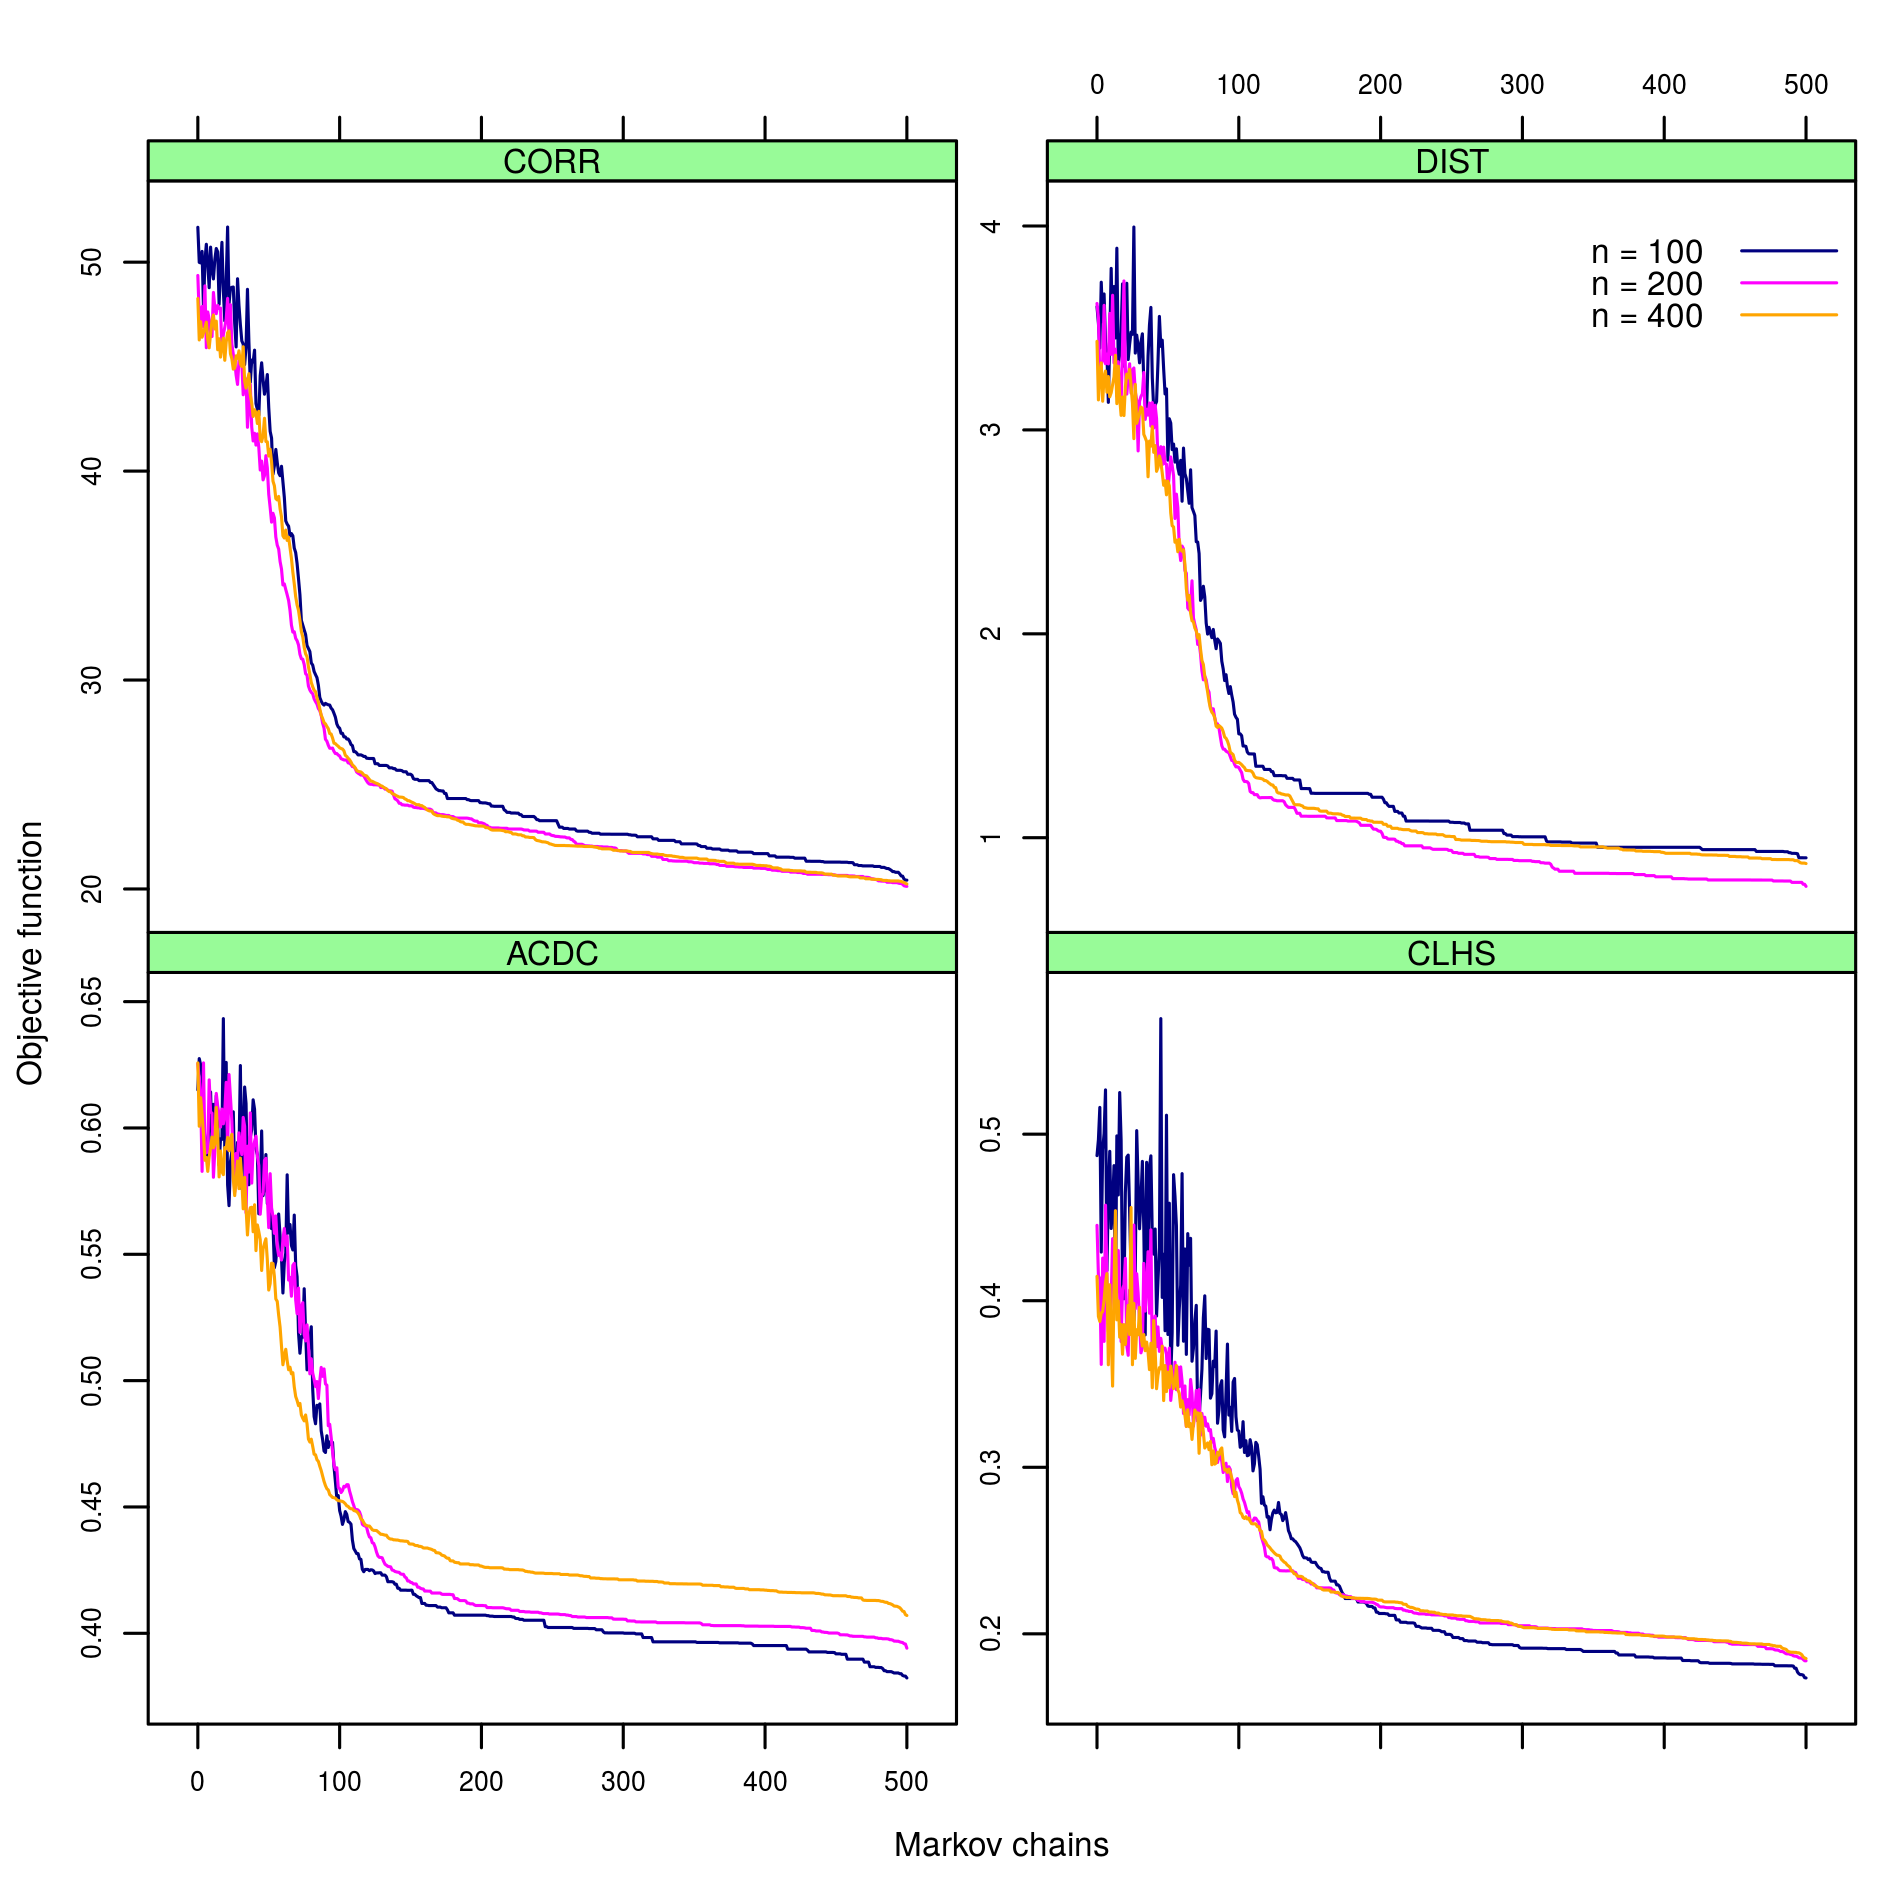
\includegraphics[width=0.90\textwidth]{fig/chap08-energy-corr-dist-acdc-clhs}
\caption[Objective function values during the optimization of three sample configurations using four sampling 
algorithms.]{Objective function values during the optimization of sample configurations of sizes $n = (100, 
200, 400)$ using sampling algorithms CORR, DIST, ACDC, and CLHS against the number of Markov chains of length 
$n$.}
\label{fig:chap08-energy-all}
\end{figure}

Our expectation that the first objective of the CLHS, $\mathcal{O}_1$, which aims at the marginal distribution 
of the numeric covariates, would have a numerical dominance over the second and third objective functions, 
$\mathcal{O}_2$ and $\mathcal{O}_3$, which aim at the marginal distribution of the factor covariates and 
similarity between the population and sample correlation matrices of the numeric covariates, respectively, was 
confirmed as shown in \autoref{fig:chap08-energy-acdc-clhs}. Each panel in 
\autoref{fig:chap08-energy-acdc-clhs} shows the region of the feasible objective space $\mathcal{Z}$ that has 
been jointly explored by the pairs of objective functions that compose CLHS and ACDC during the optimization of 
a sample configuration of size $n = 100$. Function values obtained during the first Markov chains are 
represented by the set of points located in the upper right corner of each panel, i.e. where a large variation 
is observed (see \autoref{fig:chap08-energy-all}). As the optimization proceeds, the variation in the objective 
function values decreases, till they reach a certain stability and concentrate in a specific region of the 
criterion space $\mathcal{Z}$ (left bottom corner of each panel). Optimally, the bivariate distribution of 
function values will follow the \SI{45}{\degree} line that crosses each panel from the top right corner to the 
bottom left corner. Deviations from the \SI{45}{\degree} line are evidence of numerical dominance of one 
objective function over the other.

Comparing $\mathcal{O}_1$ with $\mathcal{O}_2$ and $\mathcal{O}_3$, we see a strong deviation from the 
\SI{45}{\degree} line as evidenced by descendent vertical point cloud on the right side of both top panels. 
This means that the sample configuration is rapidly optimized with respect to $\mathcal{O}_2$ and 
$\mathcal{O}_3$ during the first Markov chains. The bottom left panel suggests that $\mathcal{O}_2$ and 
$\mathcal{O}_3$ are optimized jointly, with a small bias towards $\mathcal{O}_3$. Most of the optimization 
efforts are spent towards $\mathcal{O}_1$, as suggested by the high point density along the horizontal axis in 
both 
top panels. Thus, the bias in the CLHS can be ordered as $\mathcal{O}_1$ > $\mathcal{O}_3$ > $\mathcal{O}_2$. 
On the other hand, ACDC appears to be unbiased as suggested by the bottom right panel. The sample configuration 
is optimized with respect to CORR and DIST jointly, approximately following the \SI{45}{\degree} line, as 
expected. These results suggest that our proposed improvements on the CLHS produced a sampling algorithm with a 
better numerical behaviour. It is worth noting that the results presented in 
\autoref{fig:chap08-energy-acdc-clhs} refer to the sample size of $n = 100$, but the same trends were observed 
with the other two sample sizes.

\begin{figure}[!ht]
 \centering
 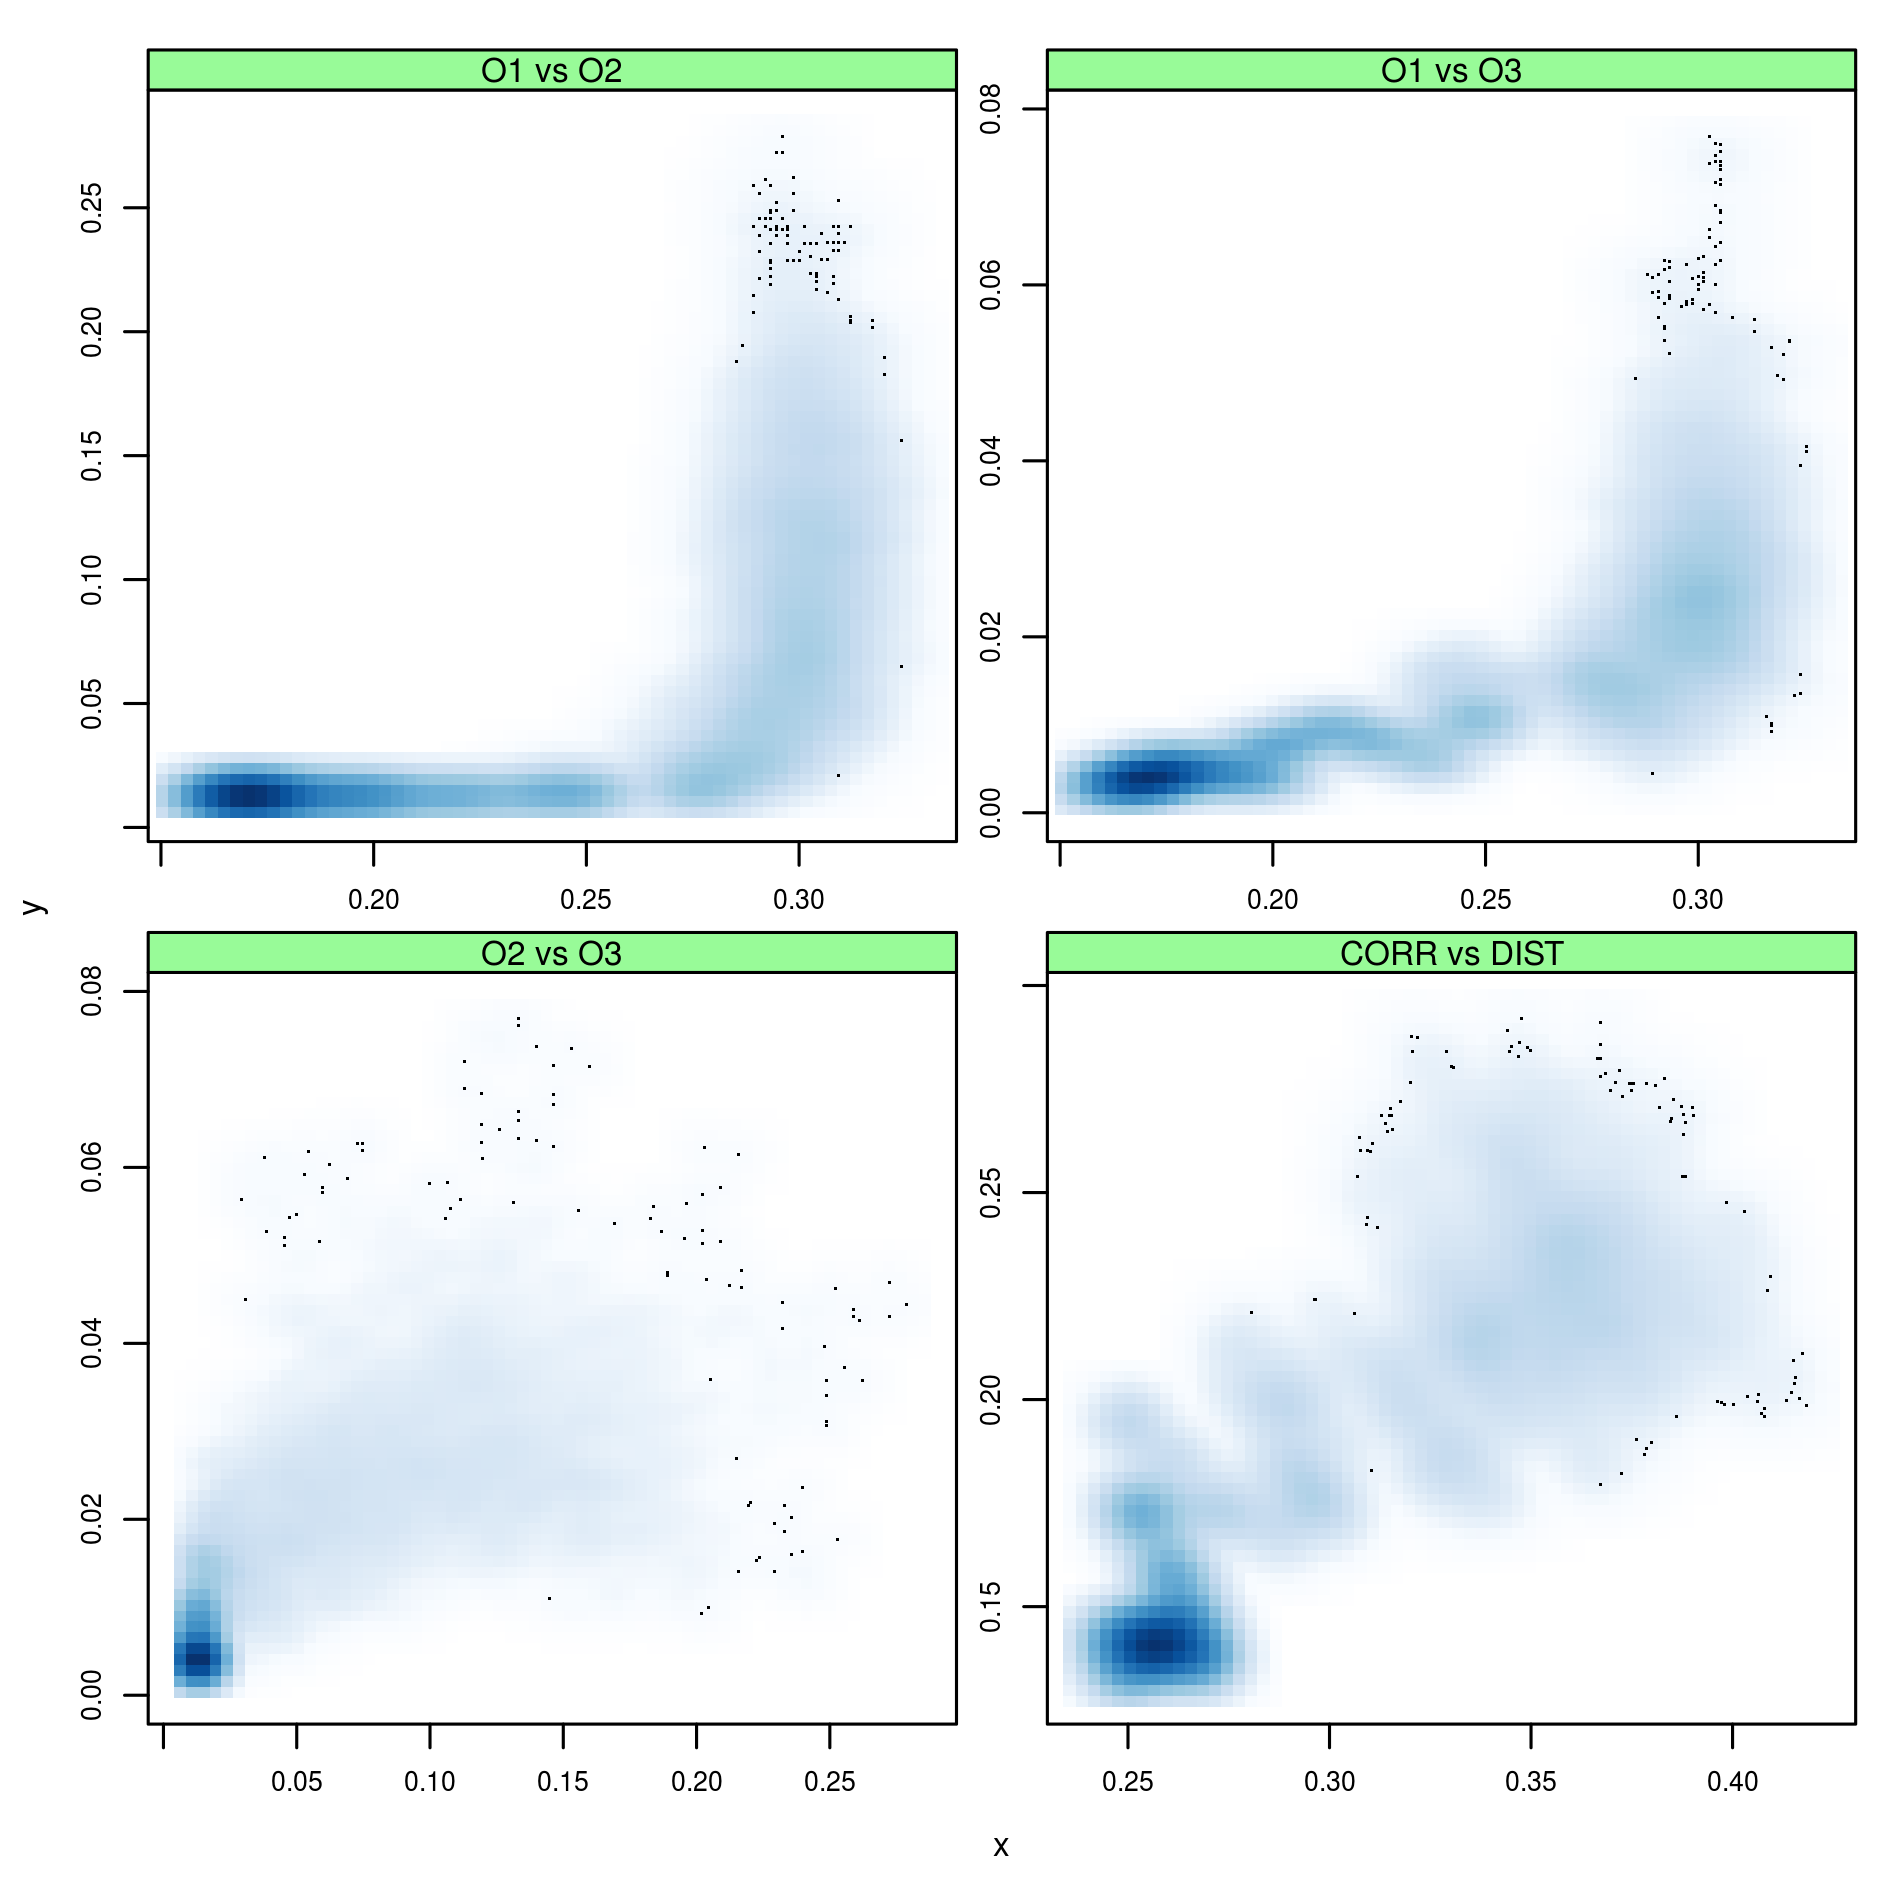
\includegraphics[width=0.90\textwidth]{fig/chap08-energy-acdc-clhs}
 \caption[Region of the feasible objective space explored by pairs of objective functions that compose CLHS 
 and ACDC.]{Region of the feasible objective space $\mathcal{Z}$ explored by pairs of objective functions (x 
 vs  y) that compose CLHS ($\mathcal{O}_1$, $\mathcal{O}_2$, and $\mathcal{O}_3$) and ACDC (CORR and DIST)  
 during the optimization of a sample configuration of size $n = 100$ using $n_{\text{chains}} = 500$ Markov 
 chains of length $n$. Darker colours indicate a higher concentration of points.}
 \label{fig:chap08-energy-acdc-clhs}
\end{figure}

A snapshot of the optimized sample configurations is presented in \autoref{fig:chap08-points}. We start by 
comparing the spatial samples produced using CORR and DIST regarding their geographic distribution. For all 
three sample sizes, DIST produces a spatial sample with a better geographic coverage, but the differences are 
smaller as the sample size increases. Since these algorithms do not aim at the coverage of the geographic 
space, leaving large spaces unsampled can have a negative effect on the prediction accuracy of calibrated 
models. CORR leaves larger empty spaces because it creates clusters of points, many of which resemble 
transects. The coverage of the geographic space of DIST samples is degraded when it is combined with CORR in 
ACDC. 
ACDC samples have more clusters of points than DIST, which again resemble transects. Both ACDC and CLHS samples 
present a similar level of coverage of the geographic space. The difference is that CLHS places clusters of 
samples in different regions than those targeted by ACDC and vice-versa. This is likely due to the numerical 
dominance of $\mathcal{O}_1$ in CLHS, which results in a bias towards numeric covariates.

\begin{figure}[!ht]
 \centering
 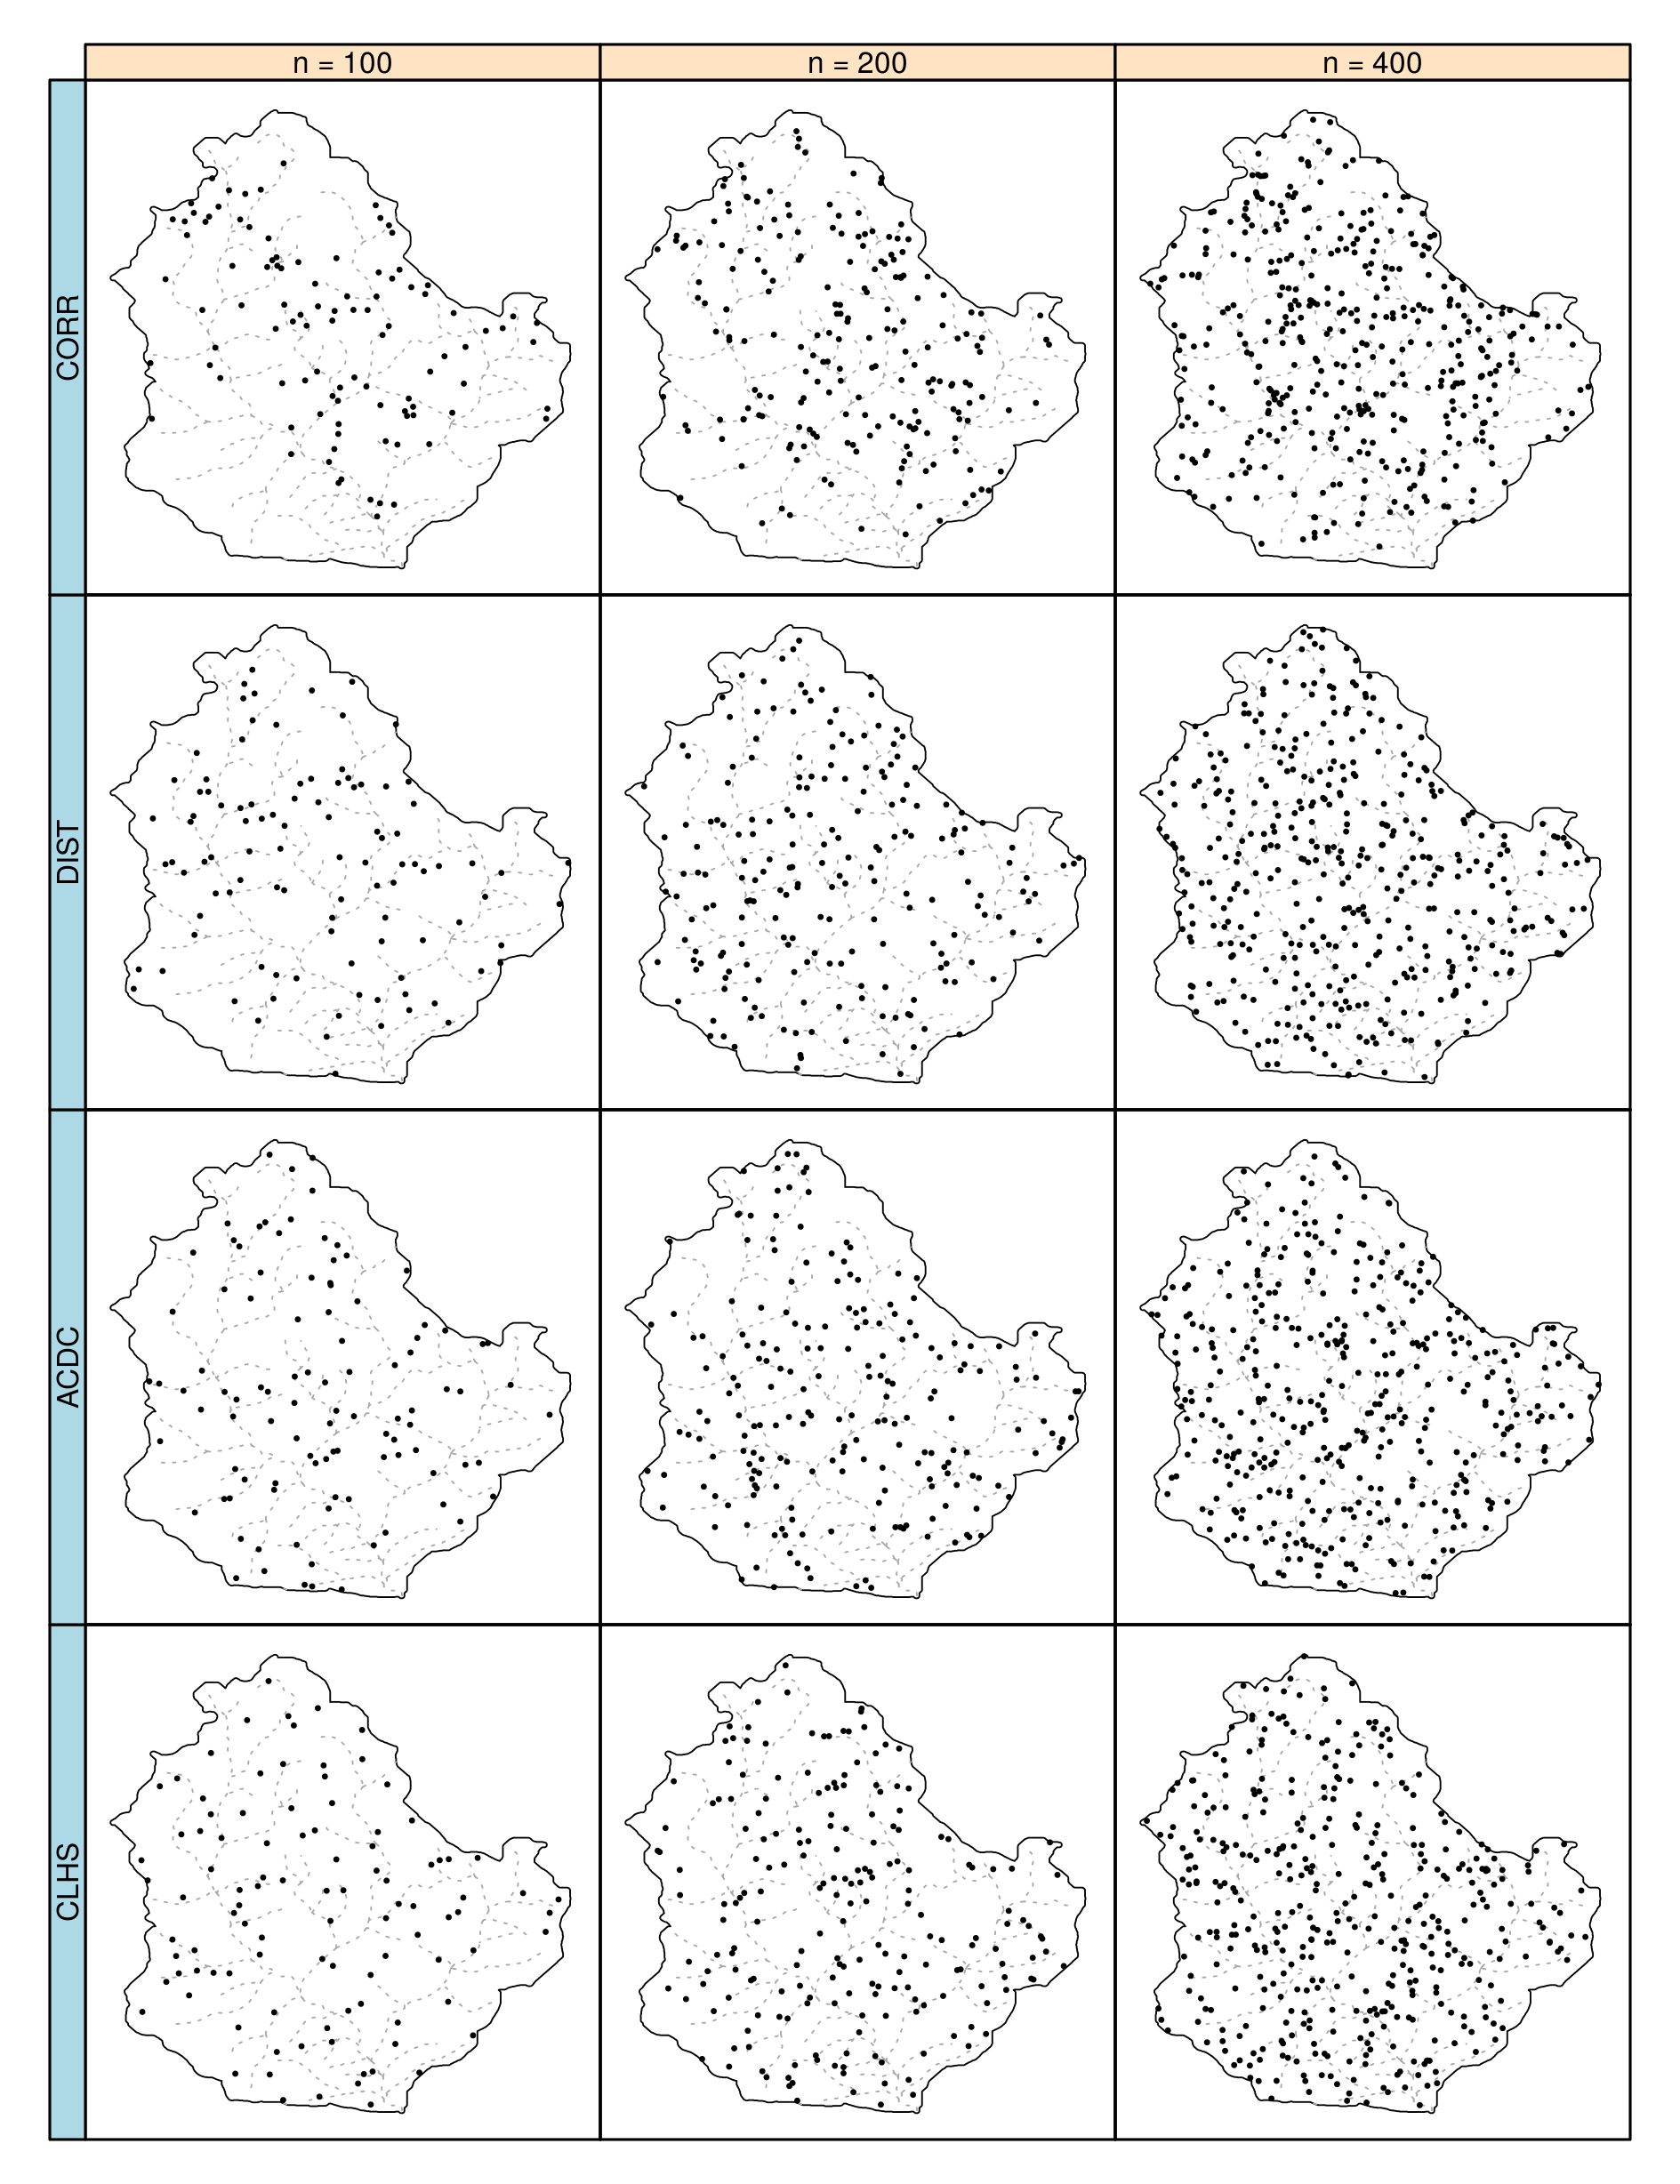
\includegraphics[width=0.90\textwidth]{fig/chap08-points-corr-dist-acdc-clhs}
 \caption[Sample configurations optimized using four sampling algorithms.]{Sample configurations of size 
 $n = (100, 200, 400)$ optimized using sampling algorithms CORR, DIST,  ACDC, and CLHS superimposing the
 drainage network.}
 \label{fig:chap08-points}
\end{figure}

Regarding prediction accuracy, as expected, increasing the sample size resulted in more accurate and precise 
predictions for all sampling algorithms (\autoref{fig:chap08-validation}). The spreads of the empirical 
distributions of all validation measures, which are approximately Gaussian, become narrower with larger sample 
sizes. The exception is the MRSE, whose distribution becomes severely skewed with $n = 400$. DIST presents the 
narrower distribution of MRSE values, but for all four sampling algorithms MRSE is above 1, which indicates 
that the prediction error variance was underestimated. This is likely because an incorrect variogram model was 
estimated with, for example, a very large nugget variance.

The CORR seems to have the largest spread of MSE values, specially for $n = 100$, suggesting that its 
predictions are the least precise. Models calibrated using spatial samples optimized using CORR consistently 
underpredicted BUDE for all sample sizes. Predictions of models calibrated with CLHS, ACDC and DIST spatial 
samples did not show a consistent bias. Together, these results suggest a degrading effect of taking the 
association/correlation between covariates into account when optimizing a sample configuration.

\begin{figure}[!ht]
 \centering
 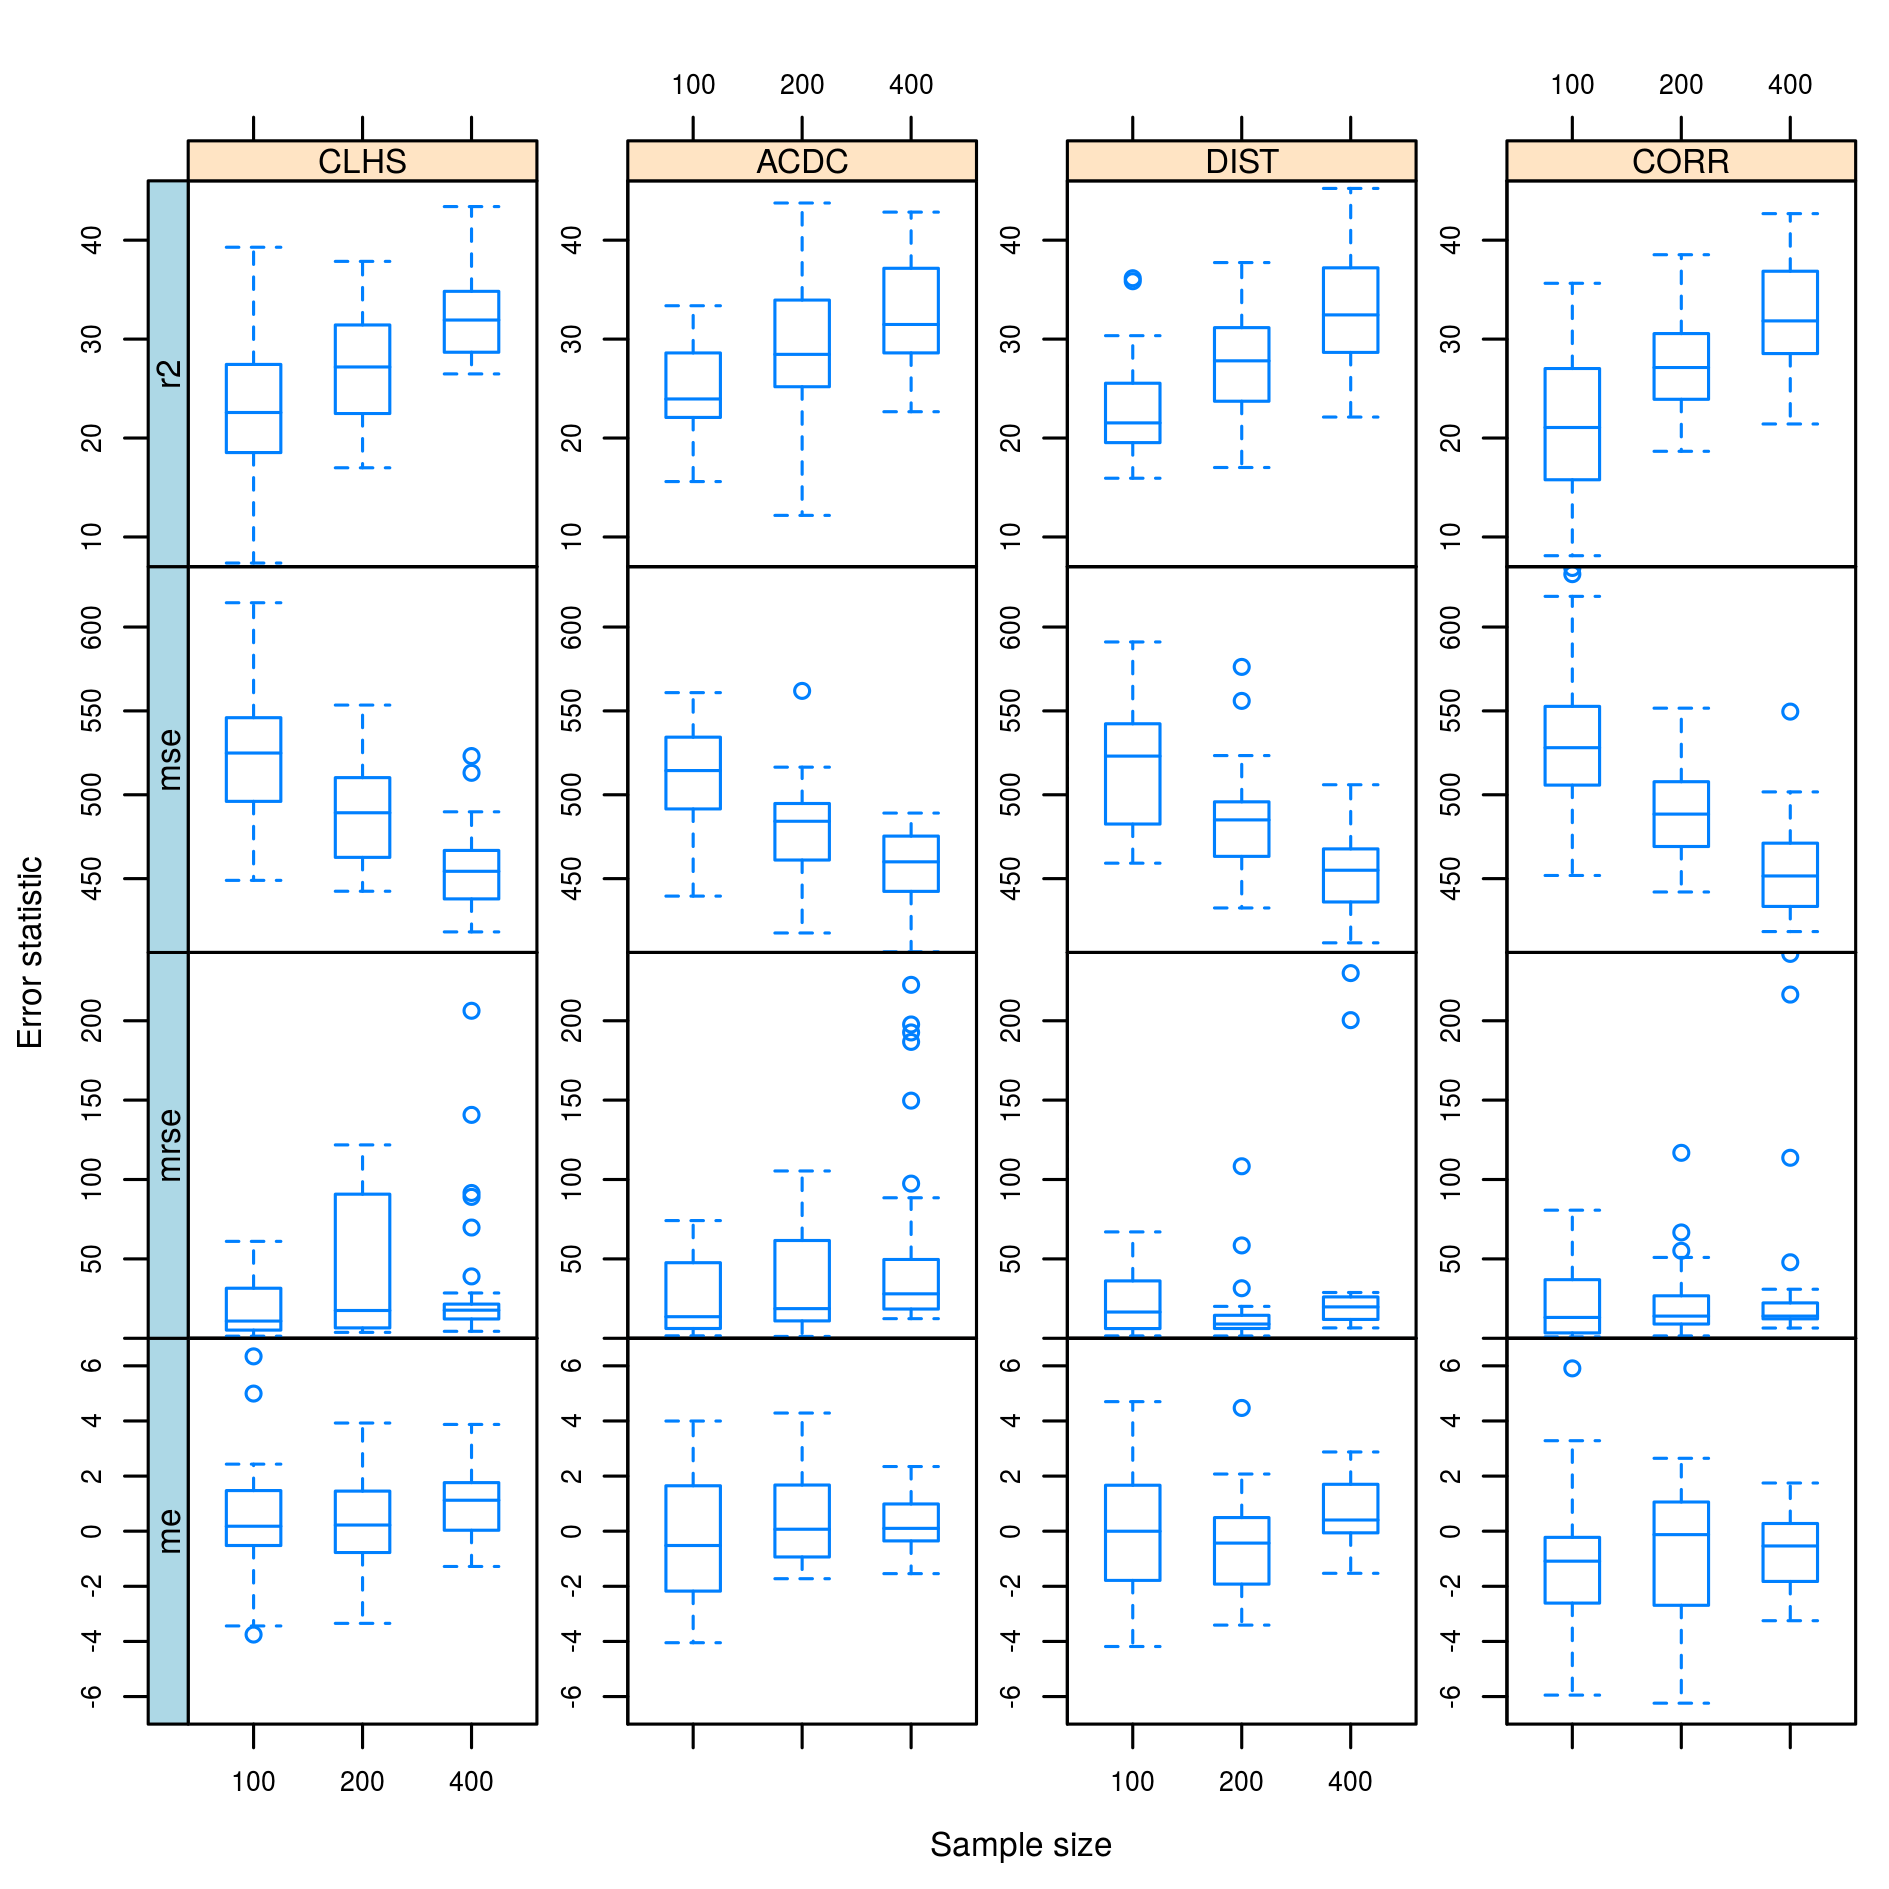
\includegraphics[width=0.90\textwidth]{fig/chap08-error-stats}
 \caption[Validation of linear mixed models calibrated using sample configurations optimized using four 
sampling algorithms.]{Statistics of the independent validation of the linear mixed models calibrated with 
simulated BUDE ($\si{\mega\gram\per\cubic\metre} \times 100$) using sample configurations with sizes $n = 
(100, 200, 400)$ optimized using sampling algorithms CORR, DIST,  ACDC, and CLHS. Statistics are the mean error 
(me), mean squared error (mse), mean ratio of squared errors (mrse), and amount of variance explained (r2).}
 \label{fig:chap08-validation}
\end{figure}

\section{CONCLUSIONS}

This study has shown that:

\begin{enumerate}[label = (\Roman*)]
\item The proposed modifications on the CLHS resulted in a sampling algorithm with an improved numerical 
behaviour, but this does not necessarily results in improved prediction accuracy;

\item Larger sample sizes improve prediction quality irrespective of the sampling optimization algorithm that
were compared;

\item Sample configurations optimized aiming only at the association/correlation between covariates can 
result in poorer predictions.
\end{enumerate}
